\documentclass[a4paper]{scrartcl}

% --- Packages ---
\usepackage[a4paper, left=1.8cm, right=1.8cm, top=2.5cm, bottom=2cm]{geometry}
\usepackage[utf8]{inputenc}
\usepackage[T1]{fontenc}
\usepackage{amsmath, amsfonts, amssymb}
\usepackage{graphicx}
\usepackage{svg}
\usepackage{float}
\usepackage{longtable}
\usepackage{booktabs}
\usepackage{adjustbox}
\usepackage{makecell}
\usepackage{threeparttable}
\usepackage{array}
\usepackage{siunitx}
\usepackage{multicol}
\usepackage{wrapfig}
\usepackage{caption}
\usepackage{algorithm}
\usepackage{algorithmic}
\usepackage{scrlayer-scrpage}
\usepackage{xcolor}
\usepackage{minted}
\usepackage{changepage}

\renewcommand{\arraystretch}{1.4}
\pagestyle{scrheadings}
\automark{section}
\ohead{\pagemark}
\cfoot{}

% --- Document Info ---
\title{SCF-PDP Programming Exercise Report}
\subtitle{Heuristic Optimization Techniques, WS 2025}
\author{
    Daniel Levin (12433760) \and
    Kartik Arya (12402369)
}
\date{}

% --- Custom Environments ---
\newtheorem{ex}{Exercise}

\begin{document}
\maketitle
% % ============================================================
% % Introduction
% % ============================================================
% \section*{Introduction}
% This assignment focuses on developing construction heuristics and local search-based metaheuristics for the SCF-PDP problem.

% \subsubsection*{Problem Description}

% The Selective Capacitated Fair Pickup and Delivery Problem \textbf{(SCF-PDP)} involves designing fair and feasible routes for a subset of customer requests. Each customer requires transportation of goods from a pickup location to a drop-off location.

% \subsubsection*{Key Characteristics}

% \begin{itemize}
%     \item \textbf{Graph Model}: Complete directed graph $G = (V, A)$
%     \item \textbf{Nodes (V)}: Vehicle depot + pickup $(v_i^\uparrow)$ and drop-off ($v_i^\downarrow$) locations
%     \item \textbf{Arcs (A)}: Fastest travel routes between locations
%     \item \textbf{Distance Calculation}: Euclidean distance rounded up: $\displaystyle \lceil\sqrt{(x_u - x_v)^2 + (y_u - y_v)^2} \;\rceil$
% \end{itemize}

% \subsubsection*{Problem Parameters}
% In this problem, only a \textit{subset of customer requests is served}. Let $n$ be the \textbf{total number of requests} and $\gamma \le n$ the minimum number that \textbf{must be fulfilled}. A \textbf{fleet} $K$ of $n_k$ \textbf{identical vehicles} is available, each with \textbf{capacity} $C$. Every \textbf{request} $i$ has a \textbf{demand} $c_i$. A solution consists of \textbf{routes} $R_k$ for each $k \in K$, where each route is an ordered sequence of \textbf{pickup} $(v_i^\uparrow)$ and \textbf{drop-off}($v_i^\downarrow$) stops. \\\\
% \textbf{Route Properties}
% \begin{itemize}
%     \item Vehicle load never exceeds $C$
%     \item Every served request is completed entirely by a single vehicle
%     \item Total number of served requests across all routes is at least $\gamma$. 
% \end{itemize}
% A fairness weight $\rho$ controls how serving decisions are balanced across vehicles.

% \subsubsection*{Objective Function}

%\[Minimize: \sum_{k\in K} d(R_k) + \rho \cdot (1 - J(R))\]

% Where:
% \begin{itemize}
%     \item $d(R_k)$: Total travel duration of vehicle $k$
%     \item $J(R)$: Jain fairness measure = $\displaystyle \frac{(\sum d(R_k))^2} {n_k \cdot \sum d(R_k)^2}$
% \end{itemize}

\section{General Setup}
\subsection{Implementation Environment}
The implementation is developed in Python 3.13. The following external libraries are utilized:
\begin{itemize}
  \item \texttt{numpy} -- efficient array operations and numerical computations
  \item \texttt{scipy} -- pairwise matrix computation of Euclidian distances via \texttt{cdist}
  \item \texttt{pymhlib} -- metaheuristic framework providing the base \texttt{Solution} and \texttt{SA} classes
\end{itemize}

\subsection{Core Classes}\label{core_classes}
The implementation consists of the following main classes:

\begin{description}
  \item[\texttt{SCFPDPInstance}] Parses and stores problem instance data including the number of requests $n$, vehicles $n_K$, capacity $C$, minimum requests $\gamma$, and fairness weight $\rho$. Precomputes the distance matrix using vectorized Euclidean distance calculations.

  \item[\texttt{SCFPDPSolution}] Extends \texttt{pymhlib.Solution}. Represents a solution as a list of \texttt{Route} objects. Provides objective calculation combining total travel distance with the Jain fairness measure, and solution validation. It supports delta evaluation of the objective value, if the corresponding flag is passed at initialization.

  \item[\texttt{Route}] Represents a single vehicle route as an ordered sequence of location indices. Tracks served requests, route distance, and enforces capacity constraints. Supports request insertion with automatic pickup-before-dropoff ordering.
\end{description}

\subsection{Experimental Setup}

\subsubsection{Implementation Stack}
\begin{itemize}
  \item \texttt{pandas} -- tabular result aggregation and formatting
  \item \texttt{matplotlib} -- visualization and plot generation
\end{itemize}

\subsubsection{Comparison Framework Architecture}
A modular algorithm comparison framework was developed to enable systematic evaluation of different heuristics. The framework is built around the following core data structures:

\begin{description}
  \item[\texttt{AlgorithmConfig}] Encapsulates an algorithm's identity: a human-readable name, the algorithm class, and initialization parameters. This abstraction allows any algorithm conforming to the construction heuristic interface to be plugged into the comparison pipeline.

  \item[\texttt{InstanceResult}] Captures per-instance metrics: objective value, construction time, total runtime (including instance parsing), and instance metadata.

  \item[\texttt{ComparisonResults}] Aggregates pairwise comparison statistics for a given instance size: mean and standard deviation of objectives for both algorithms, percentage difference, and win/loss/tie counts.

  \item[\texttt{ExperimentSummary}] Aggregates results across all instance sizes, providing total win counts and enabling cross-size analysis.
\end{description}

\subsubsection{Pairwise Comparison Methodology}\label{algos_comparison}
The comparison proceeds as follows:
\begin{enumerate}
  \item Both algorithms are executed on each instance in the test set.
  \item For each instance, the algorithm achieving the lower objective value is recorded as the ``winner.''
  \item Statistics are computed per instance size: mean objective $\pm$ standard deviation, and percentage difference defined as \[\frac{obj(\text{Alg}_1) - obj(\text{Alg}_2)}{obj(\text{Alg}_1)} \times 100\]
  \item Results are aggregated into summary tables and visualizations.
\end{enumerate}

For randomized algorithms, multiple independent runs are performed and averaged to reduce statistical variance.

\subsubsection{Extensibility}
The framework can be extended beyond pairwise comparison:
\begin{itemize}
  \item \textbf{Multi-algorithm comparison}: By iterating over all pairs of algorithms, a full comparison matrix can be constructed. The bar plots described in  \ref{experiment_visualization} can easily be extended by adding more algorithms into the plot of win distribution.
  \item \textbf{Within-algorithm comparison}: The same infrastructure supports comparing an algorithm with different parameters to itself (e.g., RCL size $k$) by treating each parameter configuration as a distinct algorithm.
\end{itemize}

\subsubsection{Visualization Infrastructure}\label{experiment_visualization}
A unified plotting module (\texttt{utils.py}) provides configurable two-panel figures via the \texttt{ExperimentPlotConfig} dataclass.
Standard visualizations include:
\begin{itemize}
  \item Objective value vs.\ instance size (line or bar plots)
  \item Runtime vs.\ instance size
  \item Percentage difference and win distribution across instance sizes
\end{itemize}
Plots support logarithmic scales, multiple series overlay, and automatic file export.

\subsubsection{Hardware}
All of the experiments were run on our local machines - MAC with M1 Pro Chip, 8 cores and 16Gb. For algorithms comparison multiprocessing was used to expedite the total runtime, for larger instances of the problem number of concurrent processes was limited to 2 to avoid memory explosion caused by replicating the instance related classes over multiple processes.  

\subsubsection{Runtime limits}
With the multiprocessing mentioned above, the runtime of the algorithms that converge in finite time (no \texttt{while true}) never exceeded 5 minutes, so we didn't need to impose an artificial timeout. For algorithms such as SA - the runtime is controlled by algorithm-specific parameters that were adjusted for larger instances.

% ============================================================
% 1. Deterministic Construction Heuristic
% ============================================================
\section{Deterministic Construction Heuristic}
\subsection{Idea} The greedy construction heuristic builds a feasible solution by iteratively selecting the closest unserved request to the current insertion point on each route. The routes are iterated sequentially and each route gets exactly one request per iteration. Requests are added one at a time, with pickup and dropoff locations inserted adjacently at the end of the route (before returning to depot), ensuring capacity constraints are satisfied at every step. This is a very primitive greedy heuristic that served as the baseline. The benefit of this approach is that it distributes the requests between vehicles evenly. However, as we experimented with the provided instances we noticed that the $\rho$ value is usually low so the impact of the \texttt{Jain} value on the final objective function is minor compared to the sum of distances. \\
The algorithm guarantees feasibility if a solution exists, raising a \texttt{ValueError} otherwise.

\subsection{Algorithm}
The algorithm maintains a set of served requests and iterates over all vehicle routes until the minimum required requests ($\gamma$) are fulfilled. For each route:
\begin{enumerate}
  \item Select the insertion position (end of route)
  \item Find the closest feasible request using Euclidean distance
  \item Check capacity constraint at insertion point
  \item If no feasible request exists, mark route as full and continue to next vehicle
  \item Insert pickup and dropoff locations consecutively (dropoff distance = 1)
  \item Repeat until $\gamma$ requests are served or all routes are marked as full
\end{enumerate}

The selection process iteratively excludes non-fitting requests and searches for the next closest alternative until a feasible request is found.

\subsection{Challenges}\label{parsing_optimization} When we started running the greedy construction heuristic on larger instances, we noticed that the runtime increased significantly. We first applied manual timing to the flow to pinpoint the bottleneck in the instance initialization, after which we used the \texttt{line\_profiler} tool to profile the function by line. We discovered that the distance matrix calculation implemented in pure Python is very inefficient, resulting in approximately 20 seconds of runtime for an instance of size 2000. After applying NumPy vectorized operations for calculating distances using the underlying CPython, which replaced the pure Python loops with a manual Euclidean distance calculation, the runtime dropped by a factor of ~100 (e.g.,~0.2s for an instance of size 2000). Since the largest instances provided are of size 10000, the parsing runtime for them still remained relatively high—approximately 20 seconds. To address this problem, given that we will be required to run many experiments on main instances, we integrated  \texttt{scipy.cdist} function, which optimizes Euclidean distance calculation and effectively reduces the parsing runtime for instances of size 10000 from 20 seconds to 2-3 seconds. See Figure~\ref{fig:greedy_construction} for visualization of the runtimes of instances parsing and greedy construction itself.
\begin{figure}
    \centering
    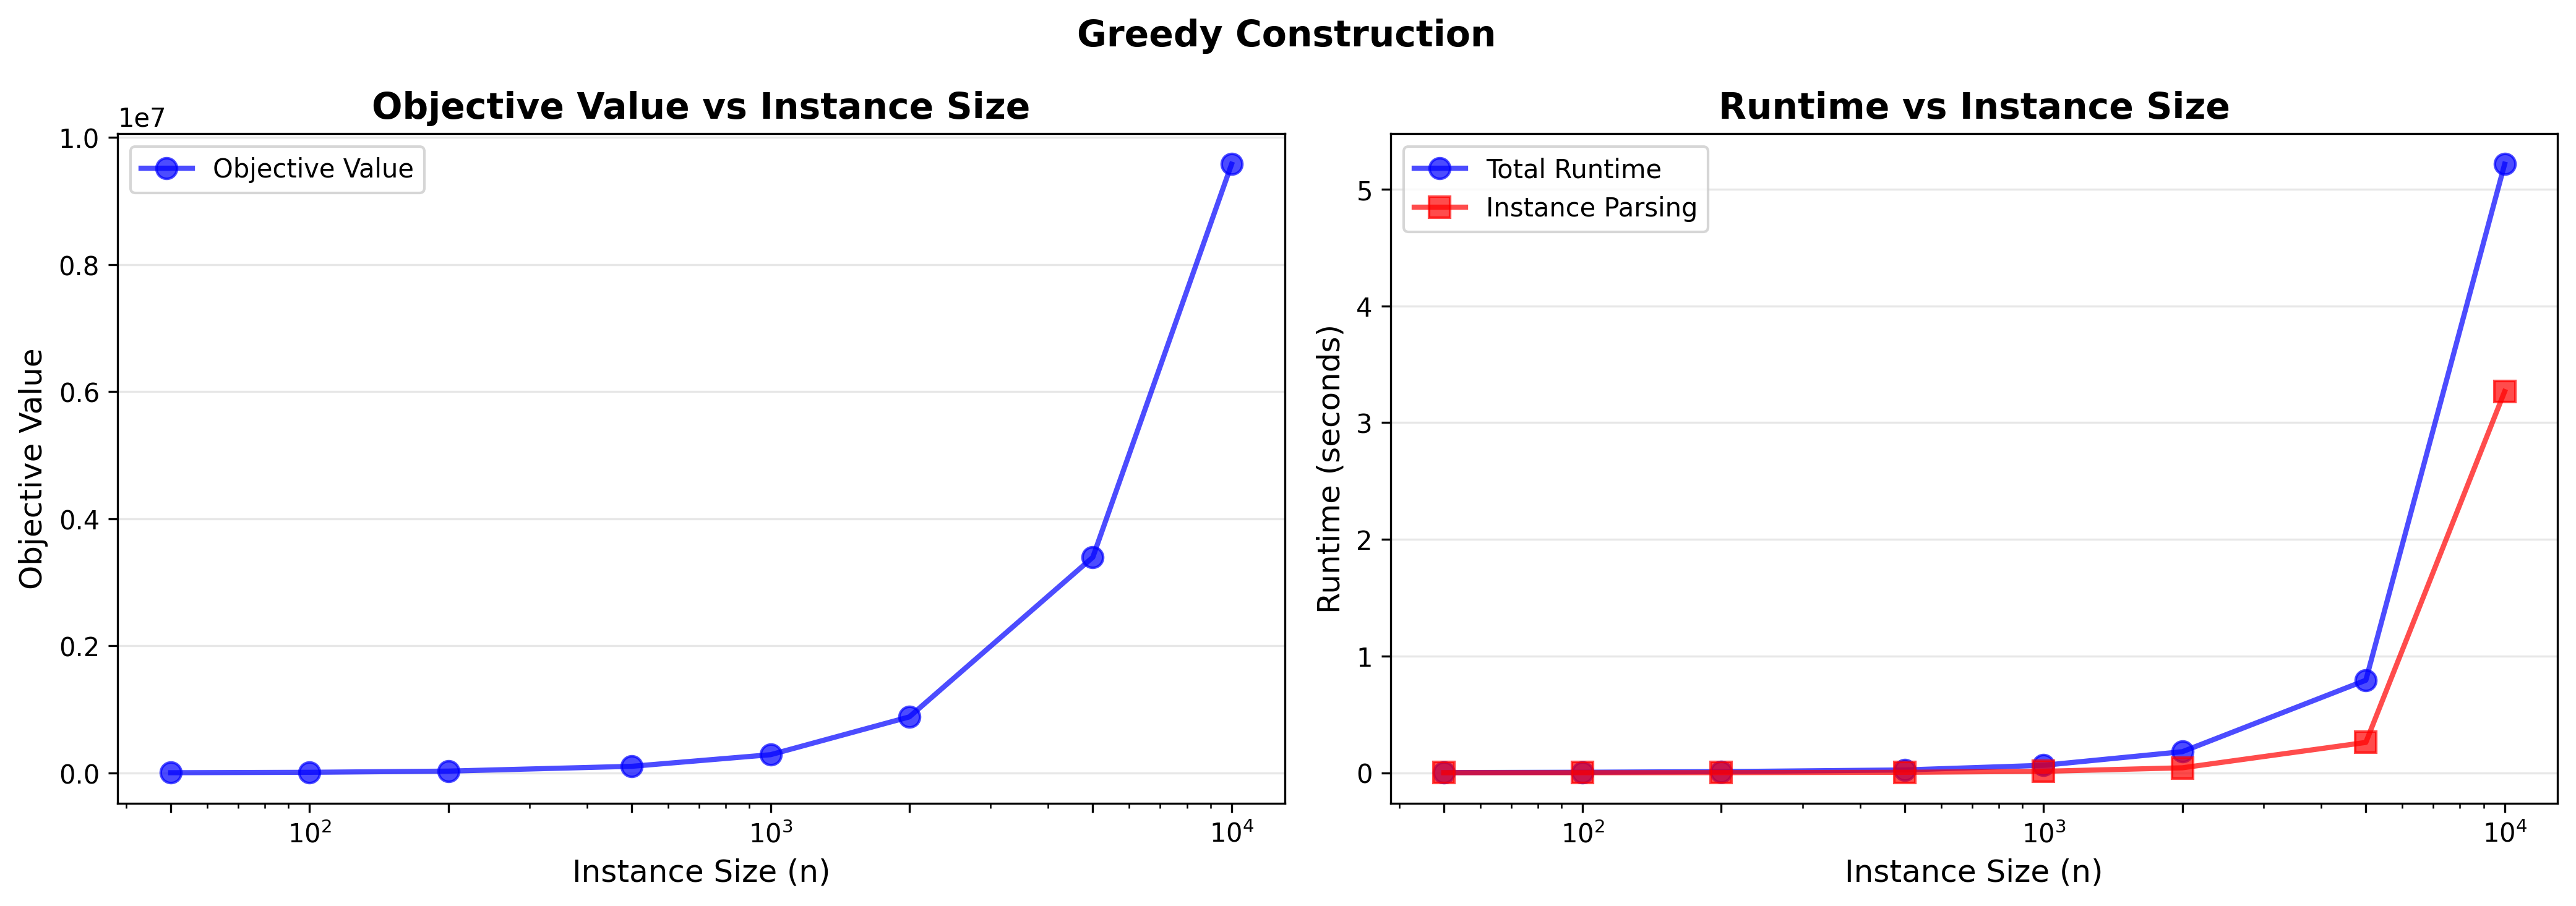
\includegraphics[width=1\linewidth]{greedy_construction_results_20251129_151821.png}
    \caption{Instances Parsing and Greedy Construction}
    \label{fig:greedy_construction}
\end{figure}

\subsection{Experiments}
Most of the experiments with greedy construction evolved around optimizing the instance parsing (see subsection~\ref{parsing_optimization}) and modeling the data structures (see subsection~\ref{core_classes}) representing evolving solutions. This work served as a baseline for all other algorithms later on. We have decided to stick to the simplest approach we came up with initially for multiple reasons:
\begin{itemize}
    \item \textbf{Simplicity} - in the beginning it was important to make sure all the classes, data structures and solution validations behave correctly and for that it was beneficial to test the simplest construction heuristic that can quite easily be cross-checked by a human.
    \item \textbf{Neighborhoods potential} - in general we wanted to find out how much exploration can different neighborhoods bring and for that it was more interesting to start with more primitive solutions instead of building promising solution by simple construction heuristic.
    \item \textbf{Time constraints} - due to the time constraints of the assignment and the number of algorithms and instances we wanted to experiment with throughout this exercise, we decided to save time on developing smarter greedy heuristics.
\end{itemize}

% ============================================================
% 2. Randomized Construction Heuristic
% ============================================================
\section{Randomized Construction Heuristic}
\subsection{Idea}
The randomized construction heuristic extends the deterministic greedy approach by introducing controlled randomness into the request selection process. Instead of always selecting the single closest feasible request, the algorithm maintains a \emph{Restricted Candidate List} (RCL) of closest feasible candidates and randomly selects among them. Feasible candidates in this case means that by adding these candidates to the chosen position on the route, the capacity constraint is not violated.

This randomization serves two purposes:
\begin{enumerate}
  \item \textbf{Solution diversity}: Different executions produce different solutions, enabling exploration of the solution space when applied iteratively (e.g., in GRASP).
  \item \textbf{Escaping greedy traps}: The purely greedy approach may lead to suboptimal solutions by making locally optimal choices that are globally poor. Randomization allows the algorithm to occasionally select non-optimal immediate choices that may lead to better overall solutions.
\end{enumerate}

The construction process remains identical to the greedy heuristic: requests are assigned to vehicles in a round-robin fashion, with pickup and dropoff locations inserted at the end of each route. The only modification is the request selection mechanism.

\subsection{Randomization Control (RCL)}
The degree of randomization is controlled through a \emph{cardinality-based} Restricted Candidate List. At each insertion step, the RCL is constructed as follows:

\begin{enumerate}
  \item Compute distances from the current insertion position to all unserved pickup locations.
  \item Filter out requests that would violate the vehicle capacity constraint.
  \item Sort remaining candidates by distance in ascending order.
  \item Select the top $k$ closest candidates to form the RCL, where $k$ is a tunable parameter \\(\texttt{top\_random\_pickups\_to\_consider}, fine-tuned default $k=10$ - see Fig.~\ref{fig:random_construction_100}).
  \item Uniformly at random select one request from the RCL.
\end{enumerate}

The parameter $k$ controls the trade-off between greediness and randomness:
\begin{itemize}
  \item $k = 1$: Equivalent to the deterministic greedy heuristic.
  \item Small $k$: Biased towards high-quality greedy choices with limited diversity.
  \item Large $k$: Greater diversity but potentially lower average solution quality.
\end{itemize}

For choosing the optimal value of \texttt{top\_random\_pickups\_to\_consider} we ran the experiments on 4 different instances with multiple \texttt{top\_random\_pickups\_to\_consider} values each, and for each of the runs we calculated the average objective value and runtime over 10 constructions. Based on the results in Figures~\ref{fig:random_construction_100},\ref{fig:random_construction_500},\ref{fig:random_construction_1000},\ref{fig:random_construction_2000} we have set the value of \texttt{top\_random\_pickups\_to\_consider} to 10 which showed stable results for every instance size. However, it is important to note that there was no consistency in objective value as the RCL size grows. This can be explained by "primitivity" of the greedy choice that the randomized version heavily relies on. Each route is a standalone TSP problem once requests for that route are fixed and a heuristic that always inserts requests in the end of the route cannot achieve good improvement in general. 
\begin{figure}[H]
    \centering
    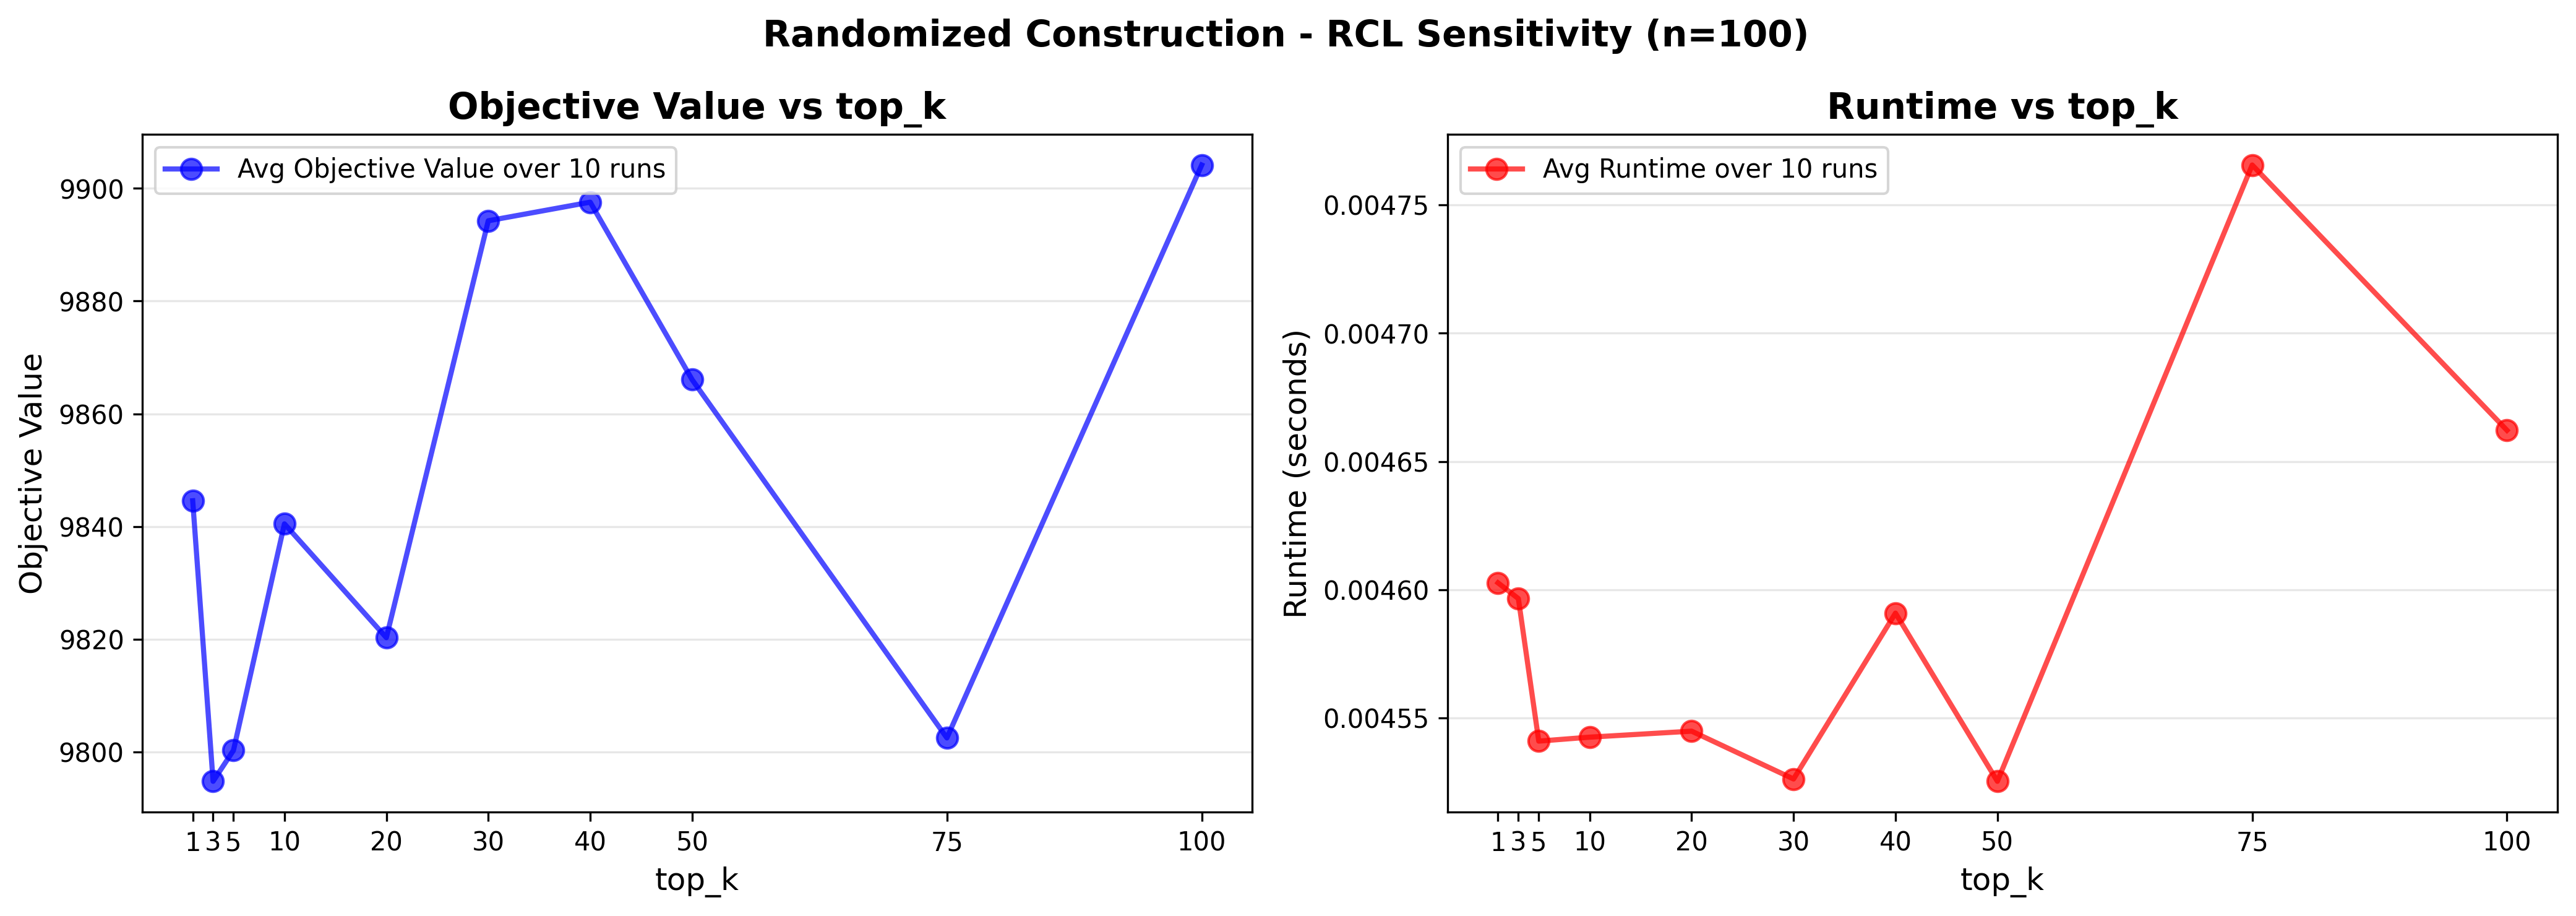
\includegraphics[width=1\linewidth]{randomized_construction_rcl_sensitivity_n100_results_20251129_164604.png}
    \caption{Random construction (n=100)}
    \label{fig:random_construction_100}
\end{figure}
\begin{figure}[H]
    \centering
    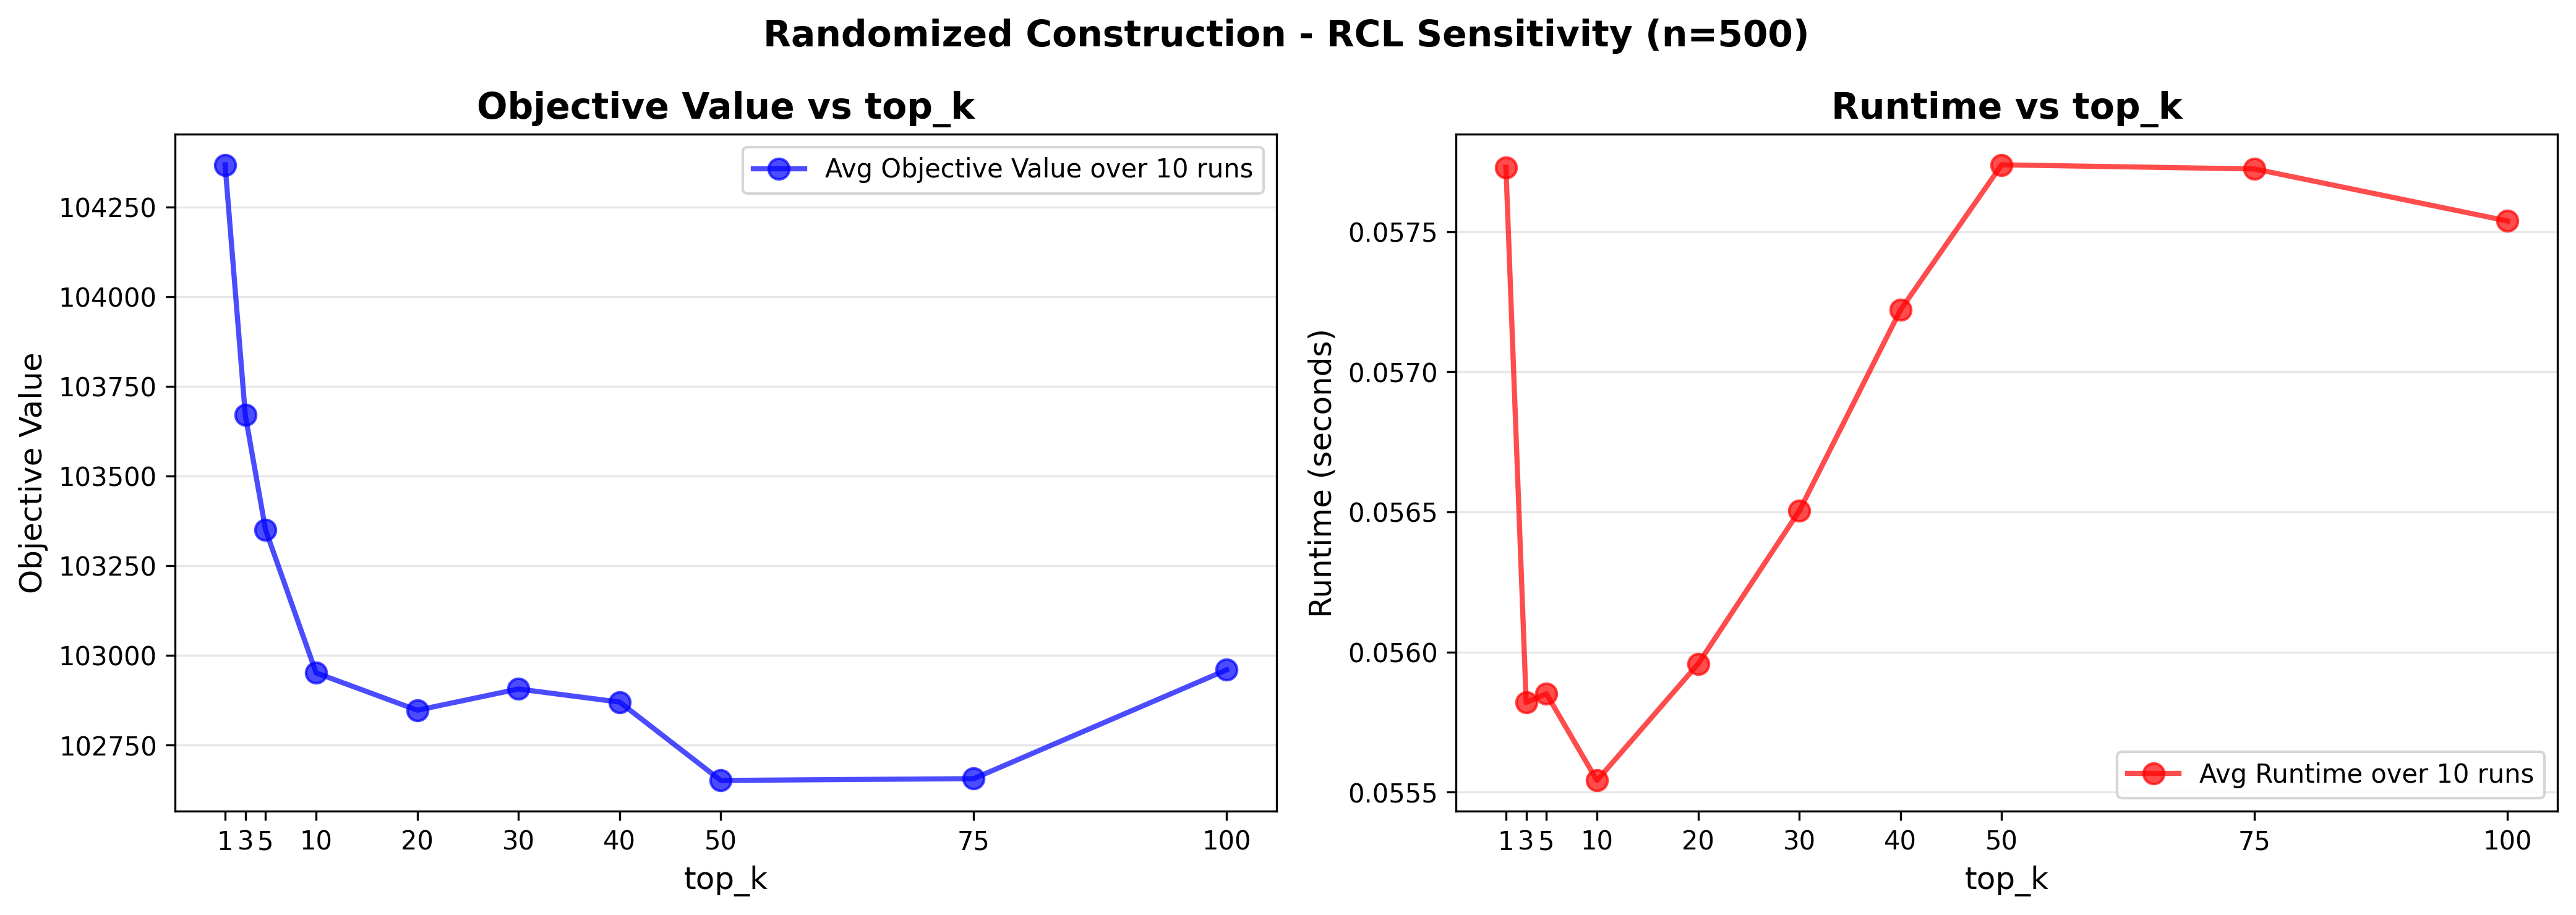
\includegraphics[width=1\linewidth]{randomized_construction_rcl_sensitivity_n500_results_20251129_164610.png}
    \caption{Random construction (n=500)}
    \label{fig:random_construction_500}
\end{figure}
\begin{figure}[H]
    \centering
    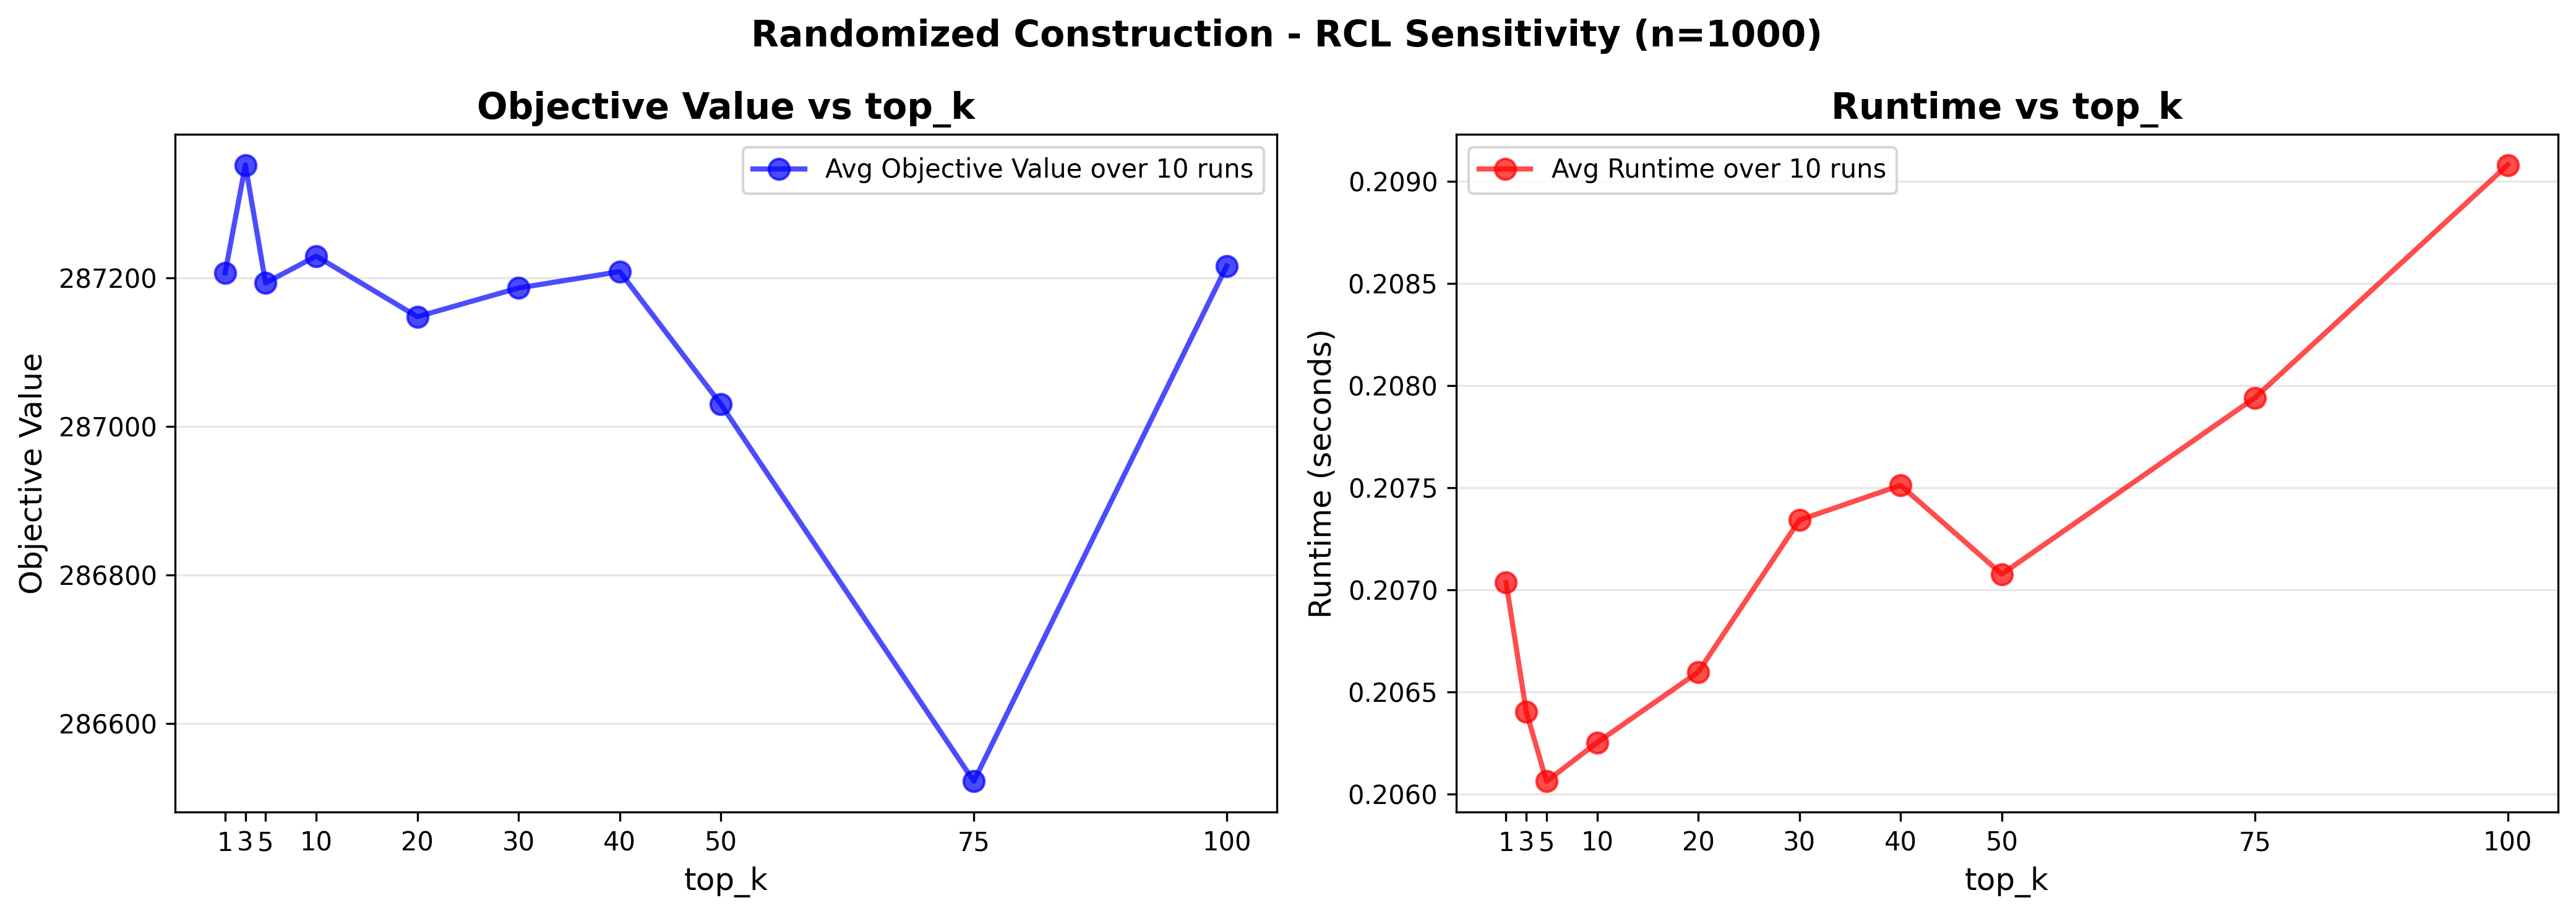
\includegraphics[width=1\linewidth]{randomized_construction_rcl_sensitivity_n1000_results_20251129_162326.png}
    \caption{Random construction (n=1000)}
    \label{fig:random_construction_1000}
\end{figure}
\begin{figure}[H]
    \centering
    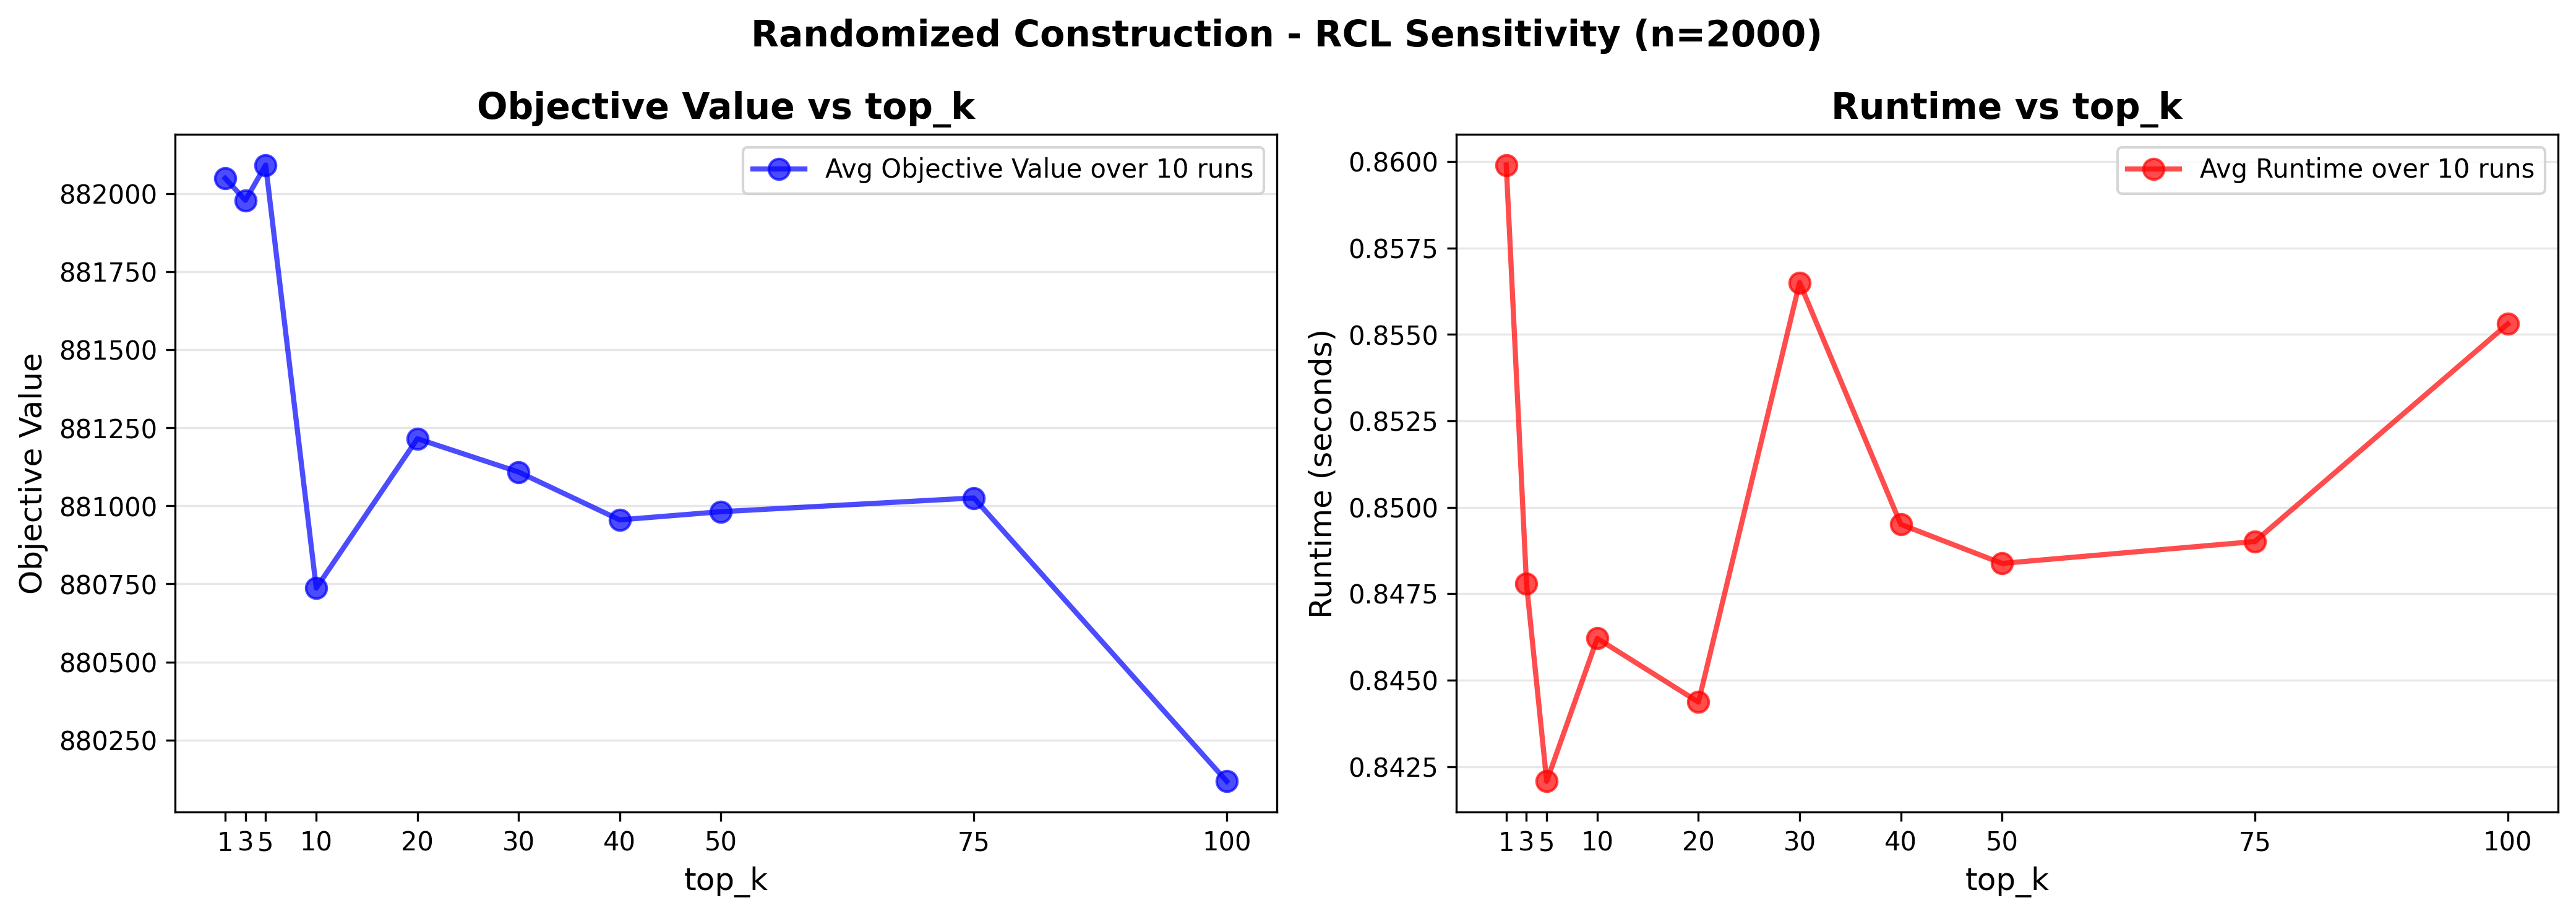
\includegraphics[width=1\linewidth]{randomized_construction_rcl_sensitivity_n2000_results_20251129_164735.png}
    \caption{Random construction (n=2000)}
    \label{fig:random_construction_2000}
\end{figure}

\subsection{Comparison with deterministic}
To compare two algorithms we built the framework described in \ref{algos_comparison} - see Fig.~\ref{fig:greedy_vs_random}. The data that these plots are based on is summarized in the table~\ref{tab:greedy_vs_random}. Every instance under the \texttt{test} folders was used for this comparison and average values were aggregated per instance size (8 average objective values per algorithm each representing 30 solution). It can be seen from both the table and the plots that on most of the instance sizes, greedy construction performs better in terms of total objective value, however, out of 240 instances it absolutely won 119, which is slightly less than half. Another interesting observation is that even when overall average of the instances of a certain size is better (=lower) for one algorithm, the number of absolute wins for that instance size of this same algorithm might be lower (see Fig.~\ref{fig:greedy_vs_random}). This can be explained by non-linear impact of single decisions of this construction approach - one wrong decision of randomized algorithm might lead to a larger gain of the objective value.
This analysis together with some experimenting we've conducted on randomized construction heuristic has brought us to the conclusion that the solutions it generates are not very diverse. The reason for that is the primitivity of the greedy construction approach randomized approach is built upon, that doesn't allow to generate more diverse routes for example with dropoffs not following the corresponding pickups strictly. However, we decided to stick to the current approach for reasons such as simplicity and time limit. 

\begin{table}[ht]
\centering
\caption{Greedy vs Randomized-$k10$ performance}
\label{tab:greedy_vs_random}
\begin{tabular}{r l l l c}
\toprule
Size & Greedy Obj & Randomized-$k10$ Obj & \% Diff & Wins (G/R/T) \\
\midrule
50     & 3399.9 ± 255.6       & 3404.0 ± 252.1       & -0.14 ± 1.66 & 14/16/0 \\
100    & 9550.4 ± 526.4       & 9558.4 ± 511.2       & -0.10 ± 1.46 & 13/17/0 \\
200    & 26951.1 ± 1478.9     & 27044.7 ± 1453.9     & -0.36 ± 0.84 & 17/13/0 \\
500    & 107992.8 ± 3909.8    & 108113.3 ± 4004.6    & -0.11 ± 0.43 & 20/10/0 \\
1000   & 301485.7 ± 8934.4    & 301531.2 ± 9020.0    & -0.01 ± 0.24 & 16/14/0 \\
2000   & 865744.6 ± 35617.7   & 865629.7 ± 35261.4   & +0.01 ± 0.14 & 12/18/0 \\
5000   & 3446920.2 ± 141250.3 & 3446515.4 ± 141514.6 & +0.01 ± 0.06 & 11/19/0 \\
10000  & 9712754.5 ± 292443.2 & 9713139.8 ± 292974.5 & -0.00 ± 0.03 & 16/14/0 \\
\midrule
TOTAL  & 434243975.3         & 434248090.3          &              & 119/121/0 \\
\bottomrule
\end{tabular}
\end{table}

\begin{figure}
    \centering
    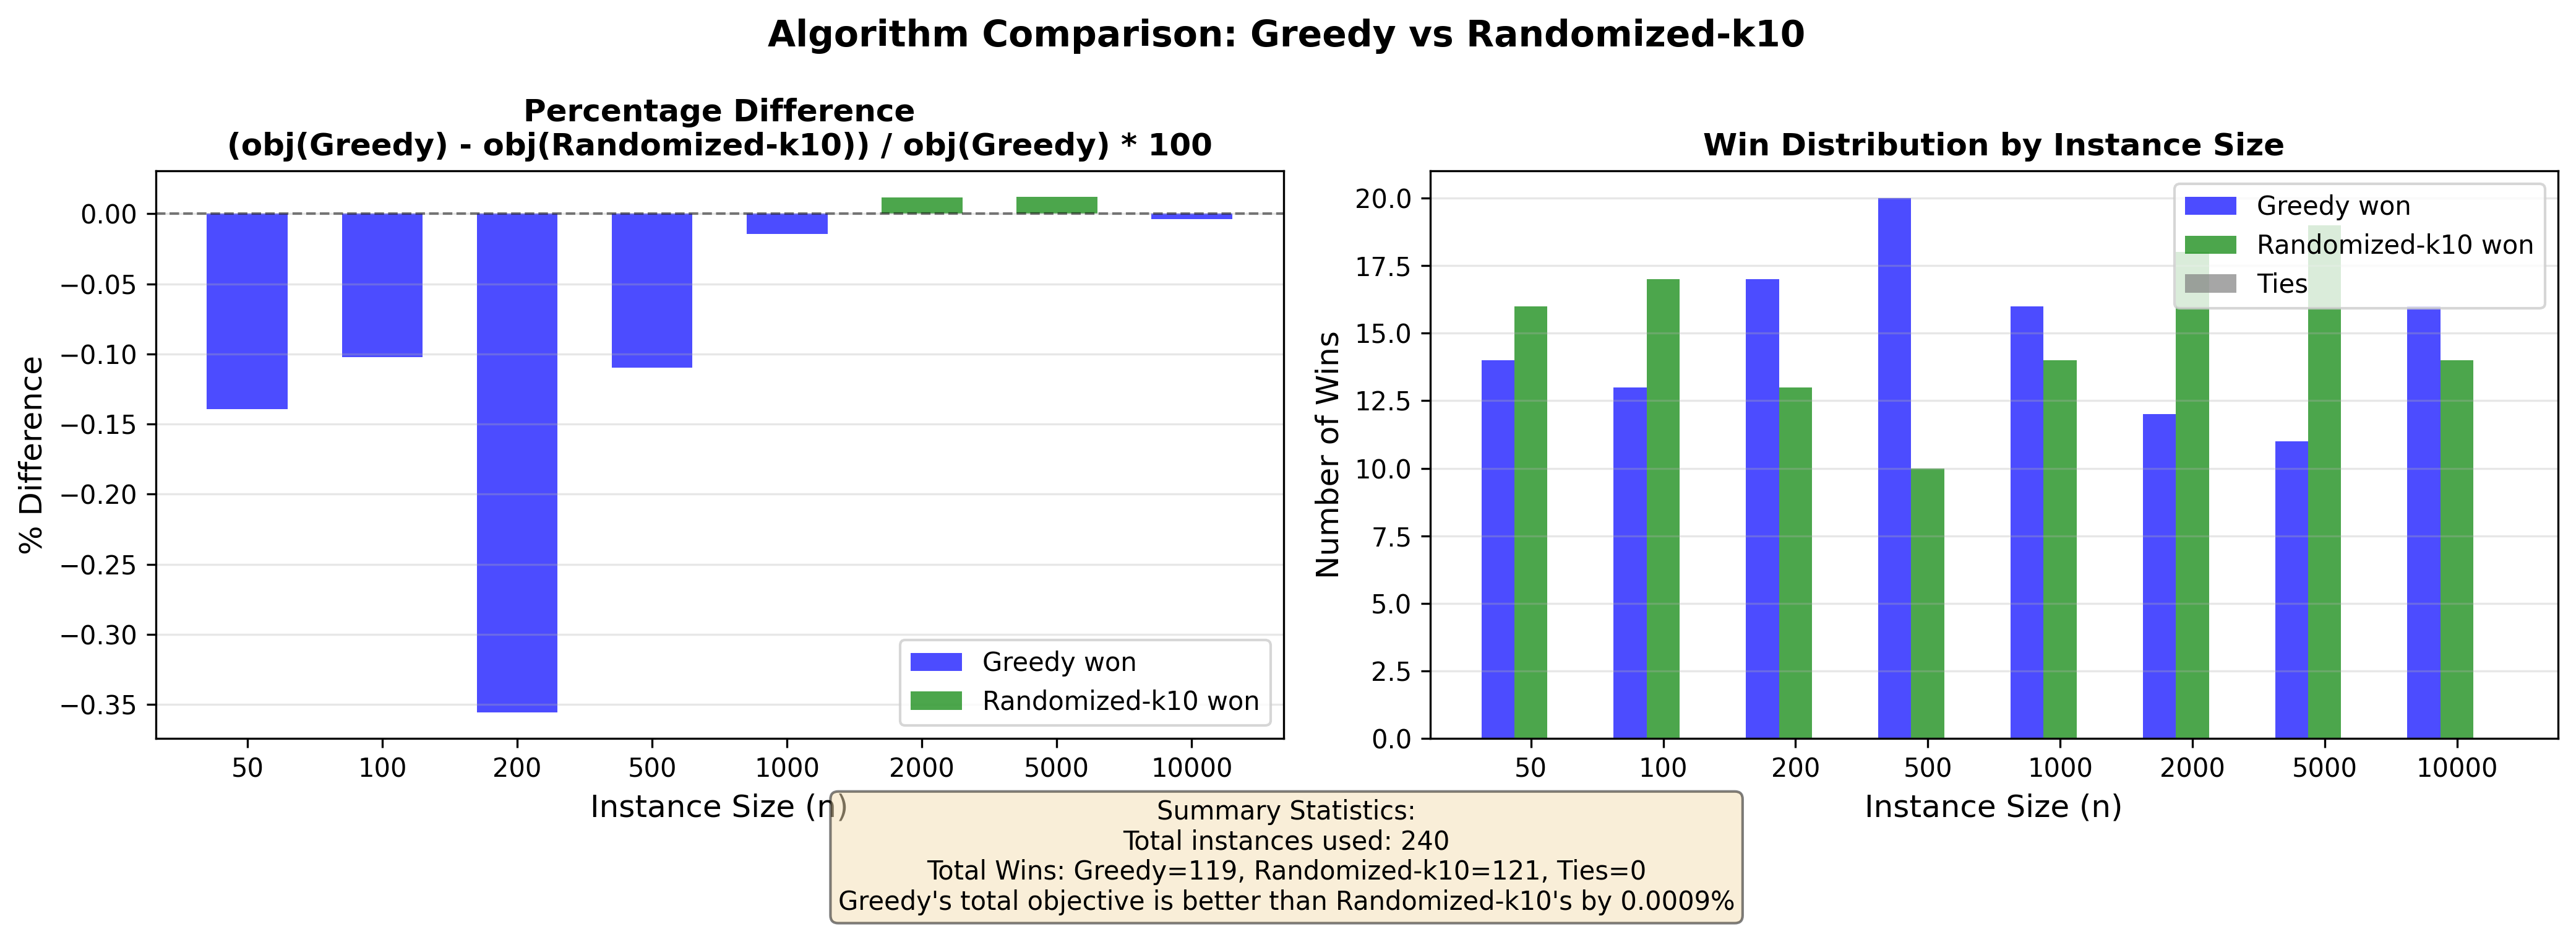
\includegraphics[width=1\linewidth]{Greedy_vs_Randomized-k10_50-100-200-500-1000-2000-5000-10000_20251129_194706.png}
    \caption{Greedy vs Randomized Construction}
    \label{fig:greedy_vs_random}
\end{figure}

% ============================================================
% 3. Beam Search
% ============================================================
\section{Beam Search Heuristic}

\subsection{Idea}
Beam search utilizes the functionality of randomized construction heuristic by maintaining multiple partial solutions (beam) during construction. The algorithm uses two key parameters: \textbf{beam width} ($\beta$) and \textbf{branching factor} (bf). Branching factor determines how many closest pickups will be conisdered at each level of the beam search. At each construction step, $\beta$ best partial solutions are kept in memory. For each partial solution, successor solutions are generated using the heuristic of the construction heuristics:
\begin{enumerate}
  \item Randomly selecting a route for extension (this has shown better results than for example choosing the route with minimal distance, although the final solution is usually less fair)
  \item Using the RCL mechanism used by randomized construction to identify a pool of closest candidate requests to branch on
  \item Creating new partial solutions by inserting different requests from the RCL
\end{enumerate}

The branching factor controls exploration breadth at each node, while beam width limits the total number of parallel solution paths considered at each step. Both insertion positions and dropoff distances are selected using the randomized construction heuristic's RCL-based selection. The algorithm terminates when all solutions in the beam are complete, returning the best solution found.
\textsc{}
\subsection{Experiments}
Parameter sensitivity analysis was conducted to determine optimal values for beam width and branching factor. The following parameter ranges were tested:
\begin{itemize}
  \item \textbf{Beam width} ($\beta$): \{2, 3, 5, 7, 10, 15, 20, 25, 30\}
  \item \textbf{Branching factor} (bf): \{2, 3, 4, 5, 6, 8, 10\}
\end{itemize}

Experiments were performed on instances of sizes $n \in \{100, 200, 500\}$, evaluating all 63 parameter combinations per instance. Results are visualized as heatmaps showing objective values and runtimes across parameter space, with optimal combinations marked (see Fig.~\ref{fig:beam_heatmap_100}~\ref{fig:beam_heatmap_200}~\ref{fig:beam_heatmap_500}). The experiments reveal the trade-off between solution quality (improved with higher $\beta$ and bf) and computational cost (increased quadratically with both parameters). Best configurations vary by instance size, with smaller instances benefiting from higher parameter values while larger instances require lower values to remain within time constraints. Interestingly, the branching factor seems to have more clear impact on the solution quality than beam width. As seen in Fig.~\ref{fig:beam_heatmap_100} for example, the largest beam width doesn't guarantee best objective value, while largest branching factor always results in best objective value across the examined configurations. This can be explained by the randomness of underlying randomized construction and RCL slicing performed by the beam algorithm. Larger branching factor allows the algorithm to look into more diverse solutions thanks to larger RCL that it generates. In this case even lower beam width are able to discover promising solutions at every level of the tree. The runtime is quadratically proportional to the beam width and branching factor which can be clearly seen in the heatmaps on the right side of figures~\ref{fig:beam_heatmap_100}~\ref{fig:beam_heatmap_200}~\ref{fig:beam_heatmap_500}. As a general note, it is clear that the beam search is not very powerful - the improvement of the objective value is not significant which can be explained by weak exploration ability of beam search and underlying construction heuristic. \\

After inspecting the heatmaps, we have decided to choose $\beta = 5$ and $bf = 10$ as our final parameters, although the results might vary depending on the instance. 

\begin{figure}[H]
    \centering
    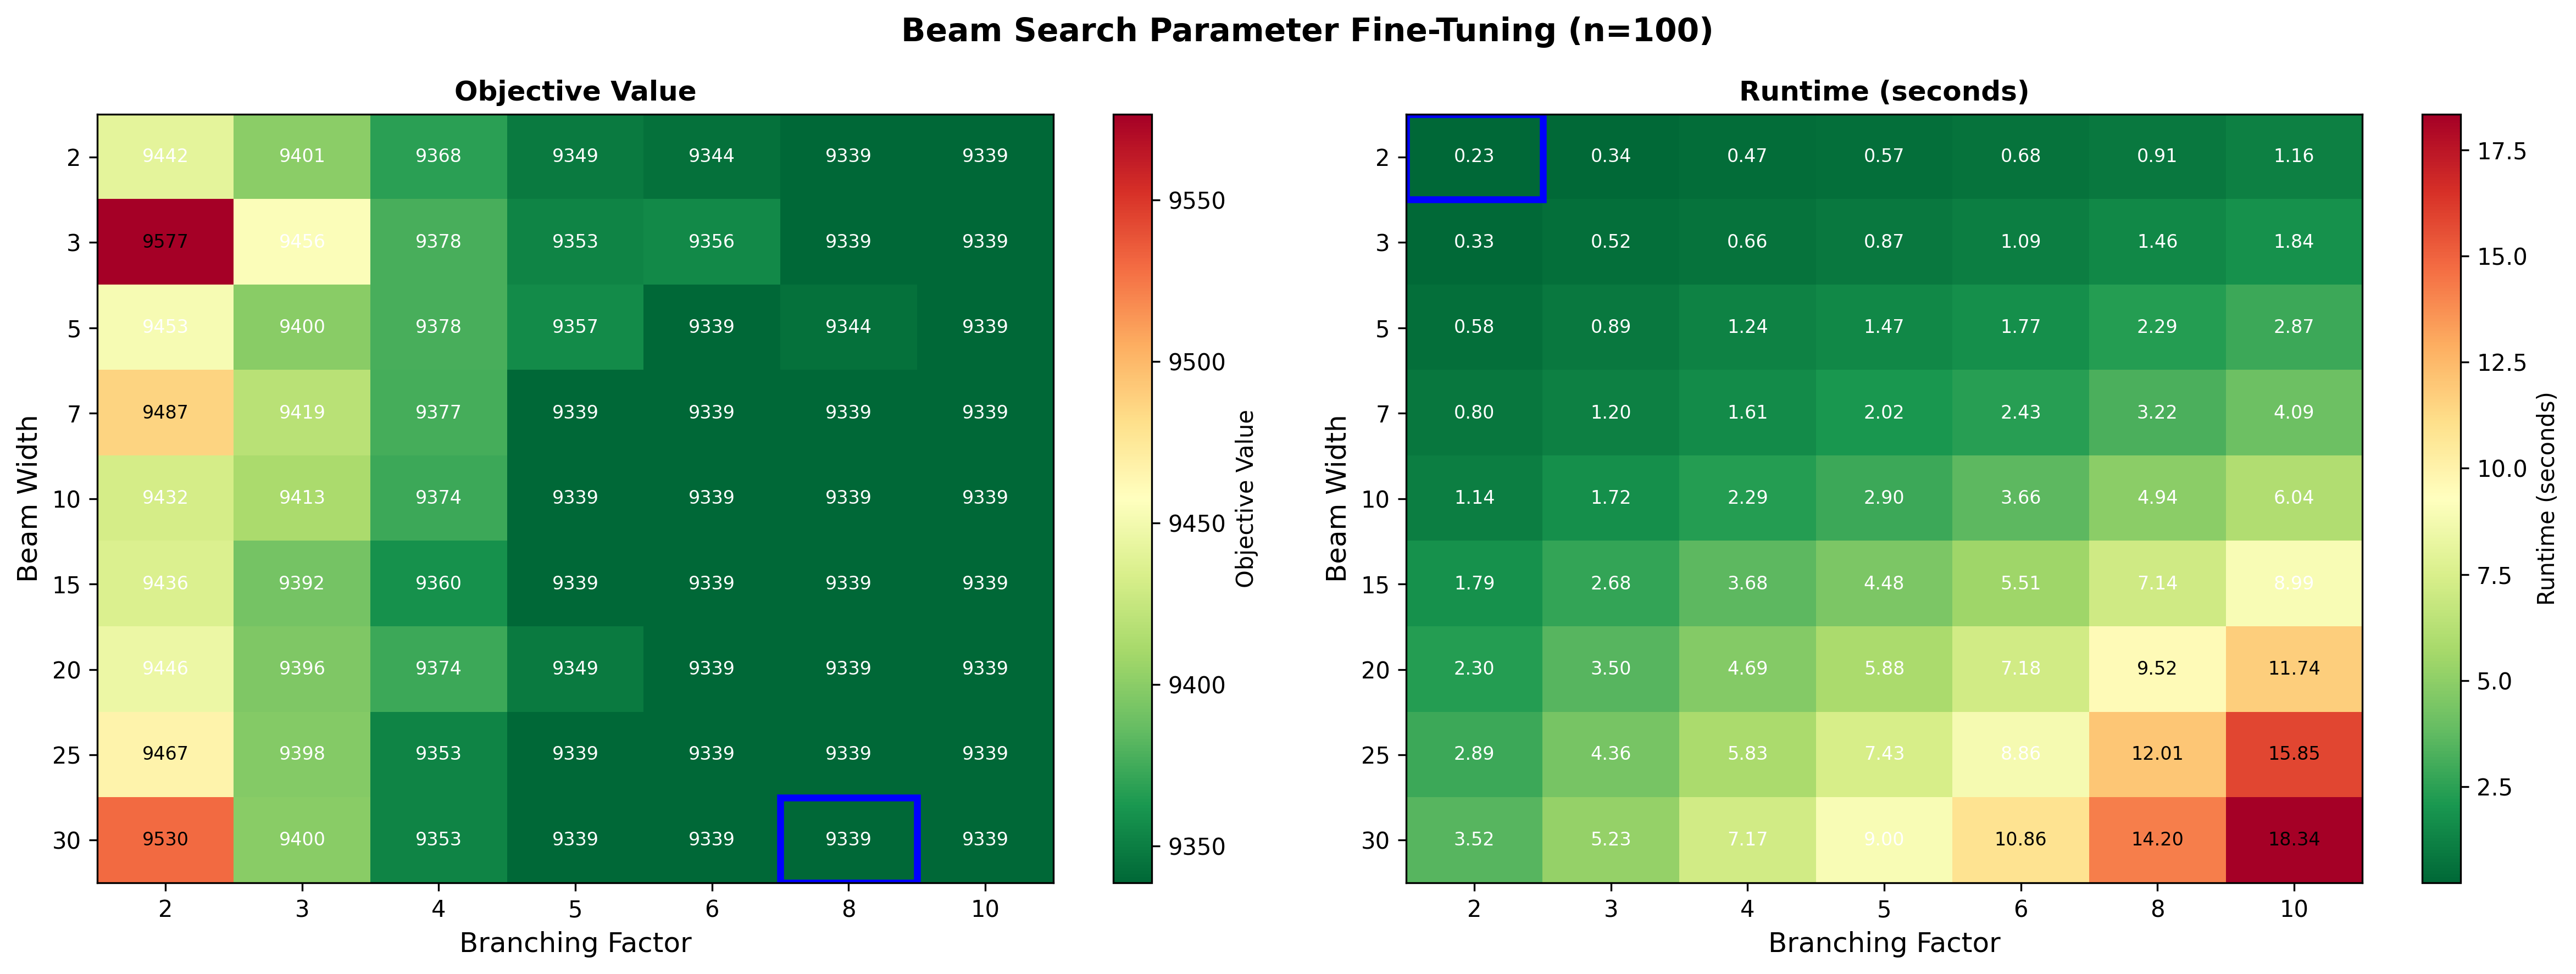
\includegraphics[width=1\linewidth]{beam_search_params_n100_20251129_220237.png}
    \caption{Beam Search (n=100)}
    \label{fig:beam_heatmap_100}
\end{figure}

\begin{figure}[H]
    \centering
    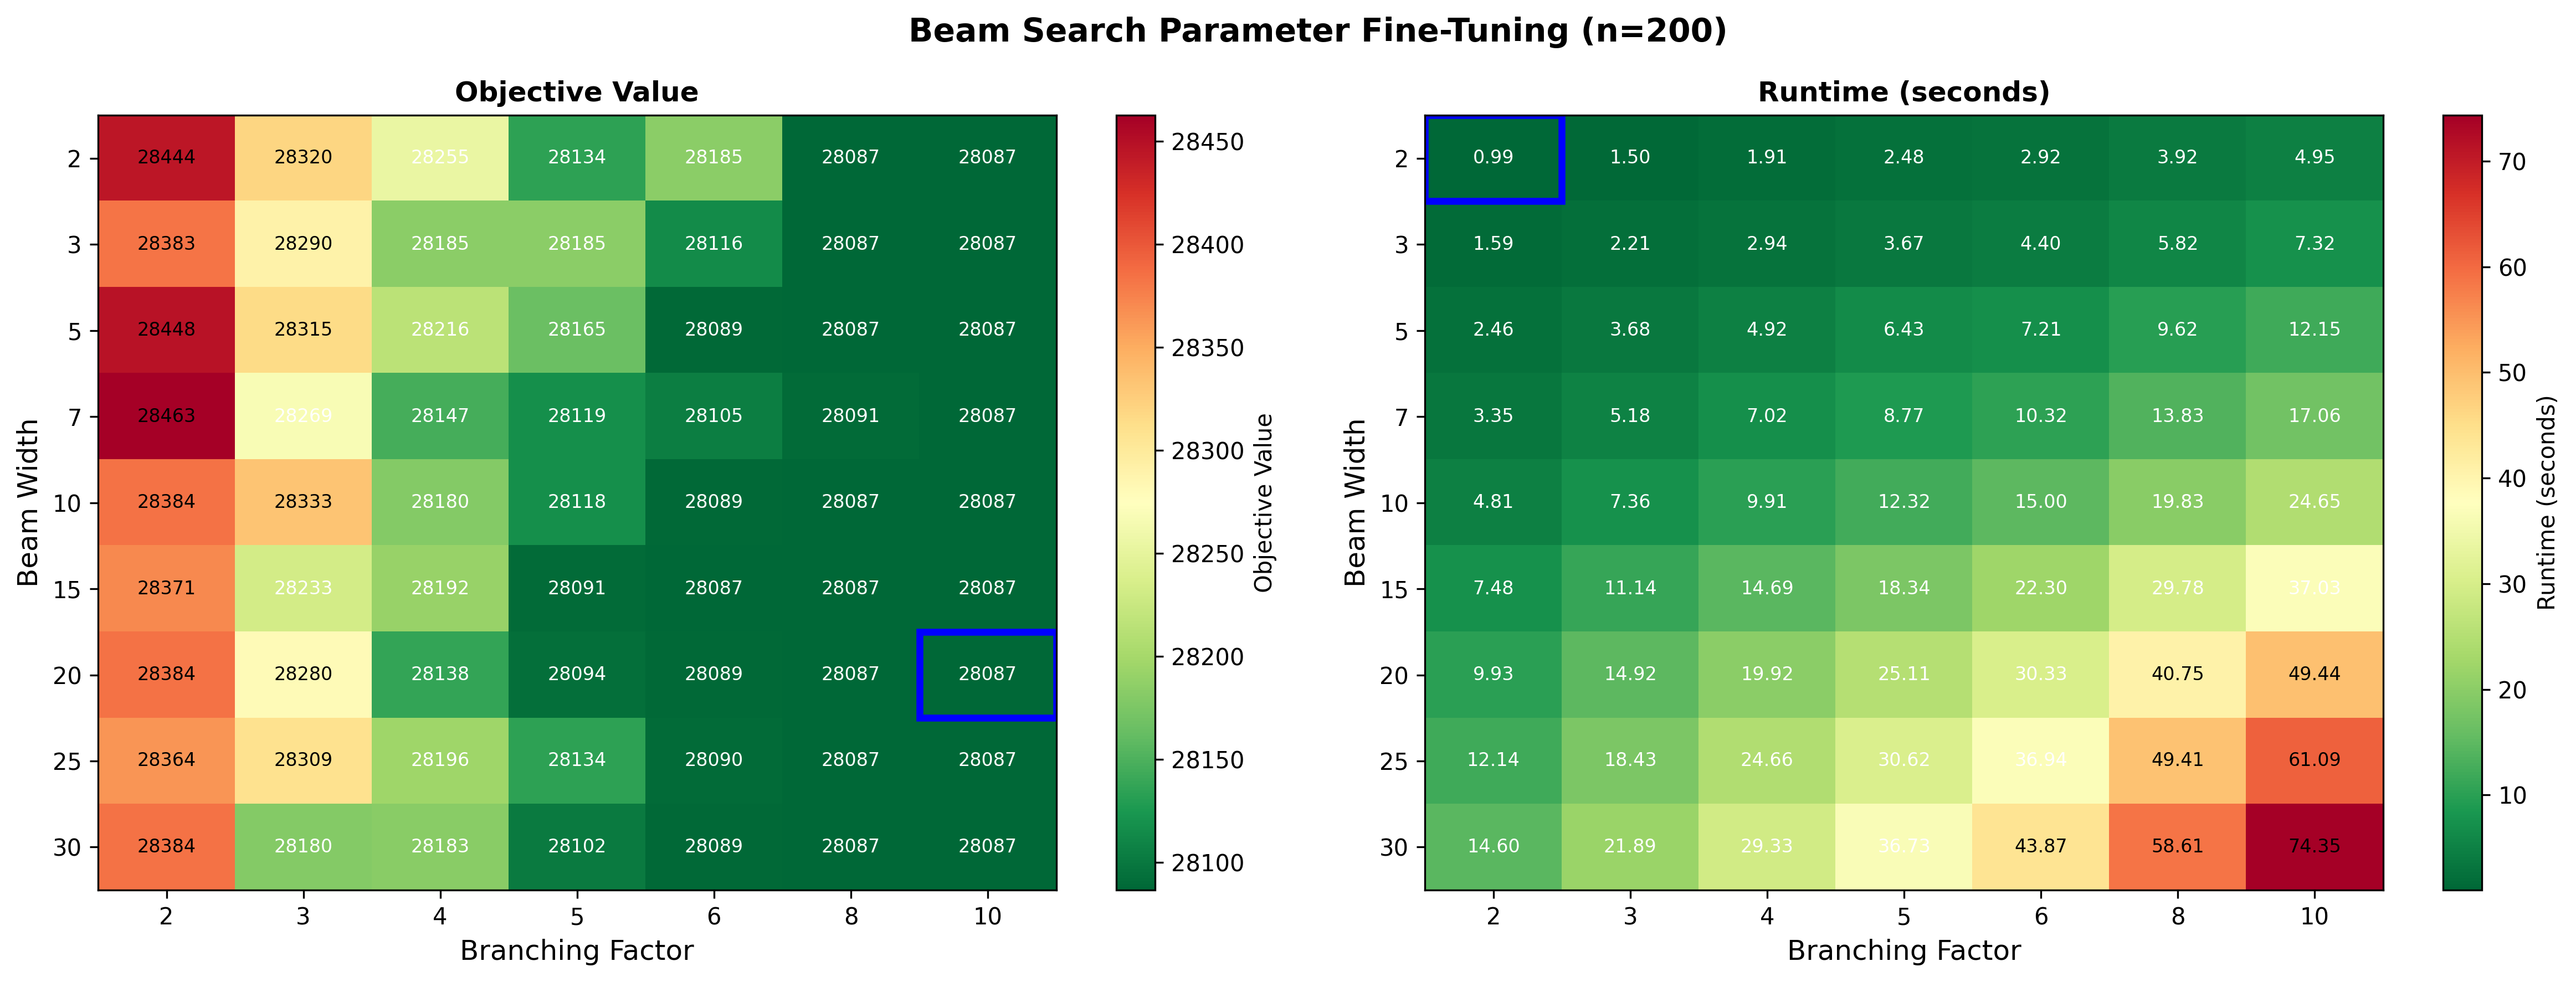
\includegraphics[width=1\linewidth]{beam_search_params_n200_20251130_001652.png}
    \caption{Beam Search (n=200)}
    \label{fig:beam_heatmap_200}
\end{figure}

\begin{figure}[H]
    \centering
    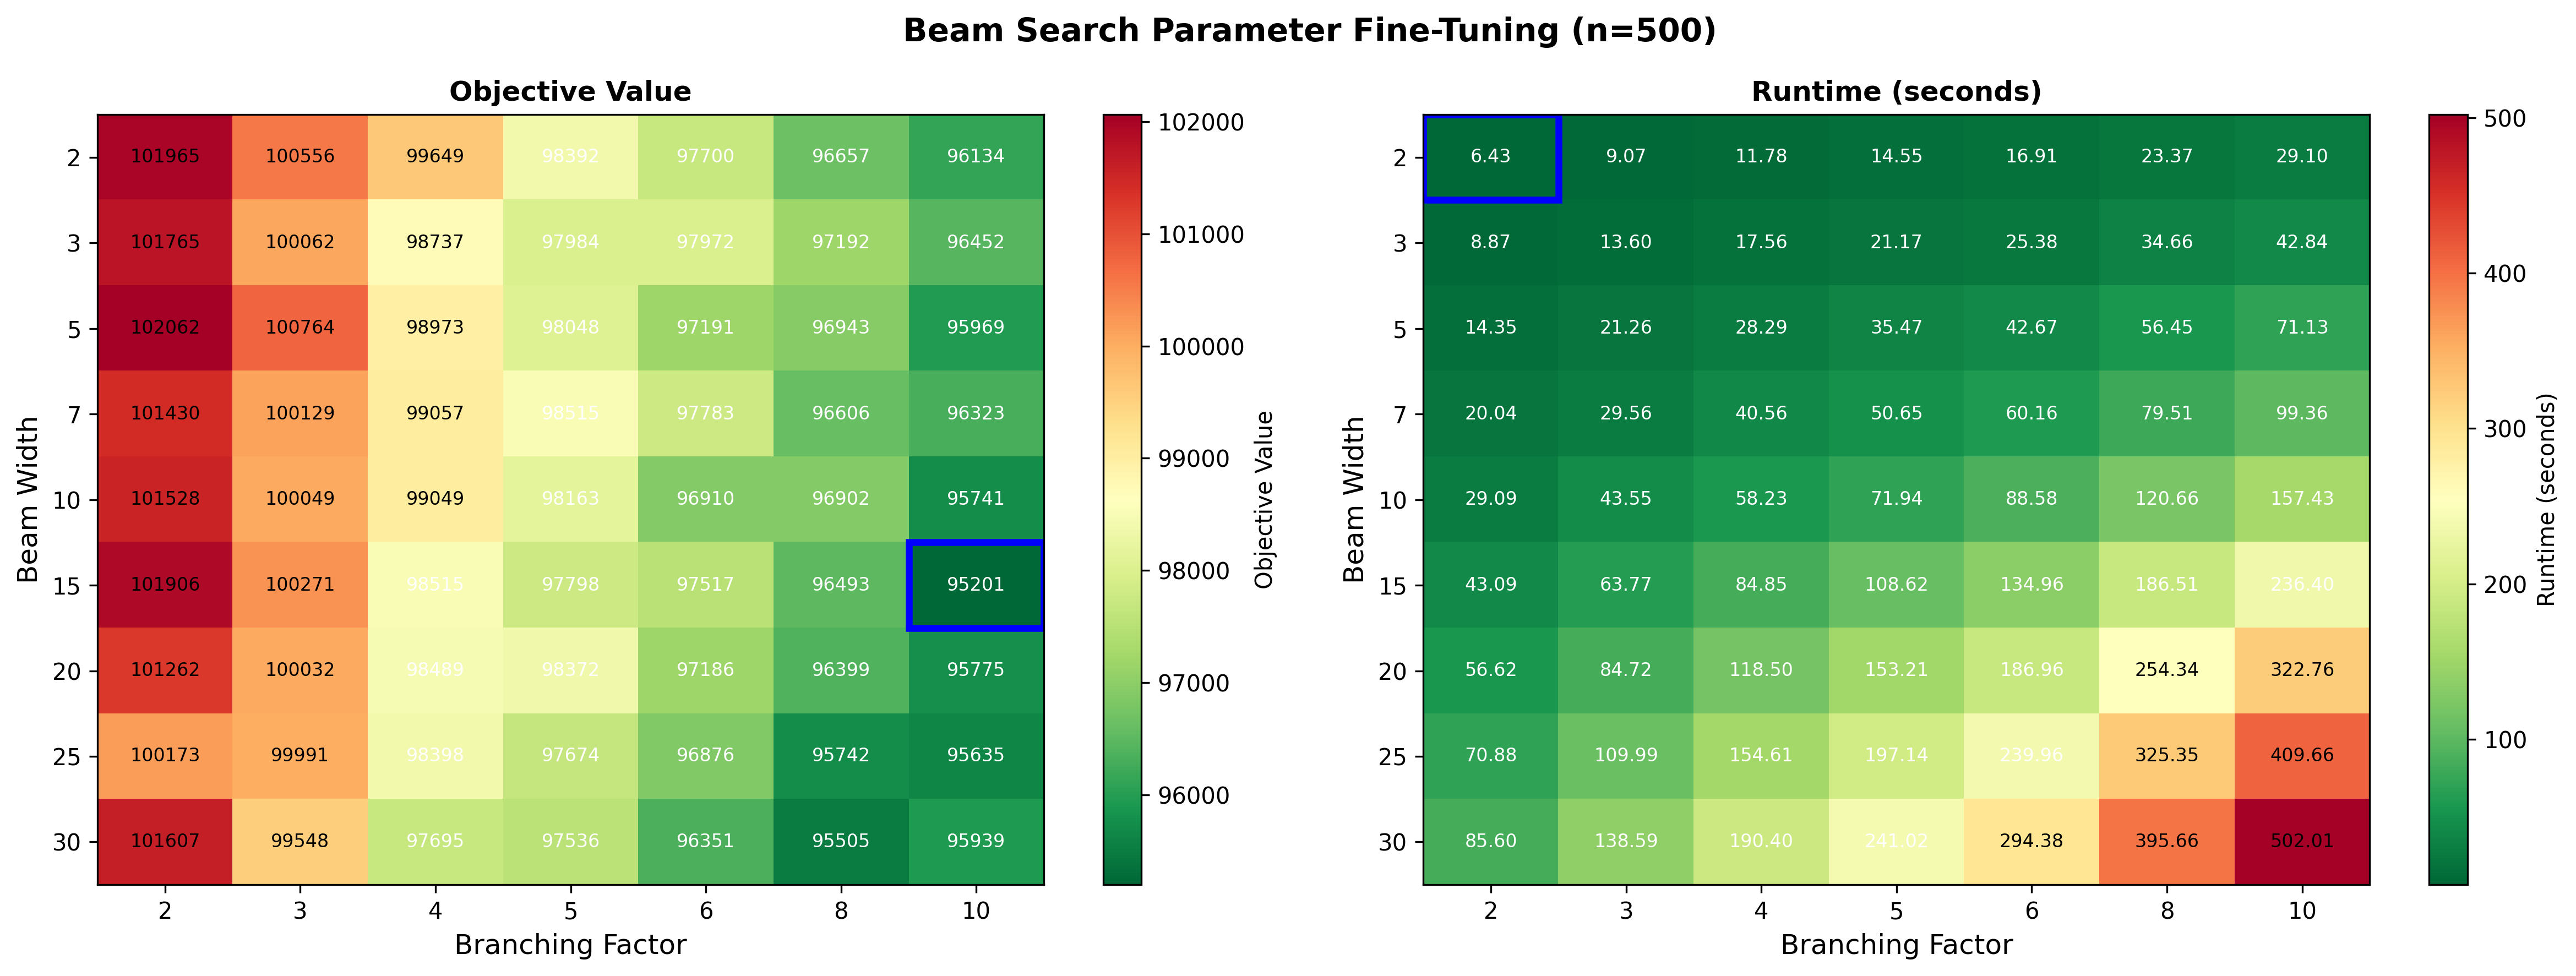
\includegraphics[width=1\linewidth]{beam_search_params_n500_20251129_235723.png}
    \caption{Beam Search (n=500)}
    \label{fig:beam_heatmap_500}
\end{figure}

% ============================================================
% 5. Local Search Framework
% ============================================================
\section{Local Search Framework}

\subsection{General Framework}

The local search algorithm operates on a current solution consisting of routes $R_k$ for all $k \in K$. It repeatedly explores a sequence of neighborhoods $\{\mathcal{N}_1, \dots, \mathcal{N}_m\}$ using a VND-style sweep. Starting from an initial feasible solution, each neighborhood $ \mathcal{N}_j $ is processed in a deterministic order. At each neighborhood:

\begin{enumerate}
    \item Apply the step strategy (\textit{first-improvement} or \textit{best-improvement}) via 
    \[
        (\text{candidate}, \text{improved}) = \text{step\_strategy.improve(current, }\mathcal{N}_j\text{)}
    \]
    \item If an improving move is found ($\text{improved} = \text{True}$), update the current solution to $\text{candidate}$ and restart the sweep from the first neighborhood.
    \item Repeat until no neighborhood yields improvement or a time limit is reached.
\end{enumerate}

This design ensures feasibility at all times (respecting vehicle capacities and single-vehicle service per request) and leverages delta-evaluation inside neighborhoods for efficiency. The repeated restart after each improvement effectively implements a VND-style search.

\subsection{Step Functions}

Two step strategies determine how neighbors are accepted during the local search:

\begin{enumerate}
    \item \textbf{First-Improvement:} Neighbors are generated lazily, and the first improving neighbor (with lower objective) is immediately accepted. This approach reduces iteration cost and quickly navigates plateaus in large neighborhoods.
    \item \textbf{Best-Improvement:} All neighbors in the neighborhood are evaluated, and the one with the best objective reduction is selected. Although more computationally intensive per iteration, this strategy provides a more stable convergence towards local optima by systematically selecting the most beneficial move.
\end{enumerate}

Both strategies are implemented through a generic interface \texttt{StepStrategy}, and can be seamlessly integrated with any neighborhood class that implements \texttt{generate\_neighbors()}. The LocalSearch class encapsulates repeated sweeps, while the VND wrapper orchestrates multiple neighborhoods in sequence.

 

% ============================================================
% 6. Neighborhood Structures
% ============================================================

\section{Neighborhood Structures}

We implement three neighborhoods that operate directly on the route representation in SCF-PDP. All use lazy generation and delta-evaluation to efficiently produce feasible neighbors.

\begin{itemize}
    \item \textbf{Insert Neighborhood.}  
    Moves a single pickup or dropoff within the same route. For route $k$, a location at $\text{pos}_{\text{from}}$ is reinserted at $\text{pos}_{\text{to}}$ using 
    $$
        \texttt{route.move\_from\_to(pos\_from, pos\_to)}.
    $$
    All valid pairs of positions are explored, generating neighbors that preserve request feasibility and capacity. This neighborhood is mainly for fine-grained reordering of stops.

    \item \textbf{Swap Neighborhood.}  
    Exchanges two stops $i$ and $j$ within the same route via
    $$
        \texttt{route.swap\_locations(i, j)}.
    $$
    It enumerates all pairs $i<j$, producing neighbors that improve route sequencing and fairness without changing which requests are served.

    \item \textbf{Relocate Neighborhood.}  
    Moves a full request (pickup + dropoff) to a different position in the same route or another route using
    $$
        \texttt{route\_from.relocate\_request\_to(request\_id, route\_to, pos\_to, 1)}.
    $$
    Iterating over all requests and possible target positions, this neighborhood redistributes workload across vehicles and adjusts fairness, enabling larger structural improvements than Insert or Swap.
\end{itemize}



% ============================================================
% 7. Variable Neighborhood Descent (VND)
% ============================================================
\section{VND Framework}

The Variable Neighborhood Descent (VND) applies a sequence of neighborhoods to iteratively improve a solution. By default, the neighborhoods are ordered as \textbf{Insert}, \textbf{Swap}, and \textbf{Relocate}, but this order can be modified if needed.

\subsection{Neighborhood Order}
VND cycles through the neighborhood list in order. Whenever an improvement is found in a neighborhood, the search immediately restarts from the first neighborhood. This ensures that early neighborhoods are fully exploited and prevents missing improvements in higher-priority moves.

\subsection{Impact of Order}
The fixed order affects convergence: placing neighborhoods that generate smaller, frequent improvements first (like Insert) allows rapid local adjustments, while larger structural moves (like Relocate) are considered later. Changing the order can alter the final local optimum and the efficiency of search.

\subsection{Stopping Criterion}
VND terminates when a complete pass over all neighborhoods fails to produce any improvement, or an optional time limit is reached. This guarantees a local optimum with respect to the entire set of neighborhoods under the selected step strategy (\textit{first-improvement} or \textit{best-improvement}).


% ============================================================
% 8. GRASP
% ============================================================
\section{GRASP}

The Greedy Randomized Adaptive Search Procedure (GRASP) iteratively constructs solutions using a randomized heuristic and improves them via local search. The procedure consists of three main components:

\subsection{Construction Phase}
A randomized construction heuristic builds an initial feasible solution. While GRASP defines a parameter $\alpha \in [0,1]$ to control greediness versus randomness, in the current implementation the heuristic selects requests randomly without actively using $\alpha$. In general, $\alpha = 0$ would yield purely greedy selection, and $\alpha = 1$ fully random selection.

\subsection{Local Search Phase}
Each constructed solution is improved using a VND over the three neighborhoods: \textbf{Insert}, \textbf{Swap}, and \textbf{Relocate}. The step strategy is \textit{First-Improvement}, though \textit{Best-Improvement} can be used as an alternative. The VND iterates through neighborhoods until no further improvement is possible.

\subsection{Iteration and Selection}
GRASP repeats the construction and local search phases for a maximum of \texttt{max\_iter} iterations. After each iteration, the solution is evaluated, and the one with the best objective value is retained. This combination of randomized construction and systematic local search allows GRASP to explore diverse solutions while converging to high-quality local optima.



% ============================================================
% 9. Metaheuristic (GVNS, SA, TS, or CC)
% ============================================================
\section{Advanced Metaheuristic (Simulated Annealing)}

\subsection{Idea}
Simulated Annealing is implemented using the \texttt{pymhlib} framework with problem-specific adaptations for SCF-PDP. The algorithm can be initialized using three construction methods: (1) beam search constructor with $\beta=10$ and $bf=4$, (2) randomized construction heuristic, or (3) greedy construction heuristic.

The neighborhood exploration uses one of three problem-specific neighborhoods:
\begin{itemize}
  \item \textbf{Insert:} Move a pickup or dropoff to a different position within the same route
  \item \textbf{Swap:} Exchange two locations within the same route
  \item \textbf{Relocate:} Move an entire request (pickup + dropoff) to a different route
\end{itemize}

At each iteration, a random neighbor is generated from the selected neighborhood. The move is evaluated using delta evaluation (see Section on Delta Evaluation) to efficiently compute the objective change $\Delta = \text{obj}_{\text{new}} - \text{obj}_{\text{current}}$. Worse moves are accepted with probability $e^{-\Delta/T}$ where $T$ is the current temperature.

Key parameters include: initial temperature $T_{\text{init}} (100)$, geometric cooling factor $\alpha (0.95)$ (applied as $T \leftarrow \alpha \cdot T$), and equilibrium iterations ($1000$) (number of iterations at each temperature level). The algorithm terminates when the maximum iteration count is reached ($10000$) or temperature becomes negligible.

\subsection{Parameter Tuning}
Parameter tuning for Simulated Annealing was performed on training instances of sizes $n \in \{50, 100, 200\}$ using the Relocate neighborhood with delta evaluation enabled. All 3 construction algorithms that have been developed were used for SA initialization via \texttt{meths\_ch} interface of the constructor. After experimenting with these constructions it was discovered that SA with Beam achieves the best objective value, albeit slower. 
\\Each configuration was evaluated across random subsample of instances in each size category of size 3, and performance was measured by mean objective value, standard deviation, and runtime. The following parameters were tuned:

\begin{itemize}
  \item \textbf{Cooling rate ($\alpha$) - see Fig.~\ref{fig:sa_alpha}:} Controls the geometric cooling schedule $T \leftarrow \alpha \cdot T$. Three values were tested: $\alpha \in \{0.90, 0.95, 0.99\}$. Higher values result in slower cooling, allowing more exploration but potentially increasing runtime.
  \begin{itemize}
      \item Best configuration: $\alpha = 0.90$
      \item Impact: Faster cooling ($\alpha = 0.90$) for some reason converged slightly slower but to better solutions. ($\alpha = 0.99$) achieved worse solution quality at the cost of longer runtime compared to $\alpha = 0.95$ and $\alpha = 0.90$. These results are counterintuitive to the SA essence because theoretically lower $\alpha$ values should result in worse solutions because the exploration is more limited - less temperatures are explored. Also in terms of the runtime - lower values should result in lower runtime because the geometric progression converges faster.
  \end{itemize}

  \item \textbf{Initial temperature ($T_{\text{init}}$) - see Fig.~\ref{fig:sa_temperature}:} Determines the initial acceptance probability for worsening moves. Three values were tested: $T_{\text{init}} \in \{50.0, 100.0, 200.0\}$. Higher initial temperatures allow more exploration early in the search.
  \begin{itemize}
      \item Best configuration: $T_{\text{init}} = 50$
      \item Impact: Low temperature ($T_{\text{init}} = 50$) behaved "greedily", which for some reason resulted in better objectives. High temperature ($T_{\text{init}} = 200$) was supposed to allow better exploration with better objective values but ended up being the worst value out of the three. The runtime didn't change significantly for different values of the $T_{\text{init}}$. This is probably due to the fact that small instances were chosen for the evaluation.
  \end{itemize}

  \item \textbf{Equilibrium iterations (equi\_iter) - see Fig.~\ref{fig:sa_equi_iter}:} Number of iterations performed at each temperature level before cooling. Three values were tested: equi\_iter $\in \{500, 1000, 2000\}$. More iterations allow better exploration
at each temperature.
  \begin{itemize}
      \item Best configuration: $equi\_iter = 500$
      \item Impact: Fewer iterations ($equi\_iter = 500$) resulted in better solution quality with slightly slower runtime. More iterations ($equi\_iter = 2000$) didn't provide improvement, neither in solution quality, nor in runtime.
  \end{itemize}
\end{itemize}

All parameter tuning experiments used a fixed iteration limit of $10000$ iterations and the Relocate neighborhood. Final parameter configuration selected: $\alpha = 0.90$, $T_{\text{init}} = 50$, $equi\_iter = 500$.

\begin{figure}
    \centering
    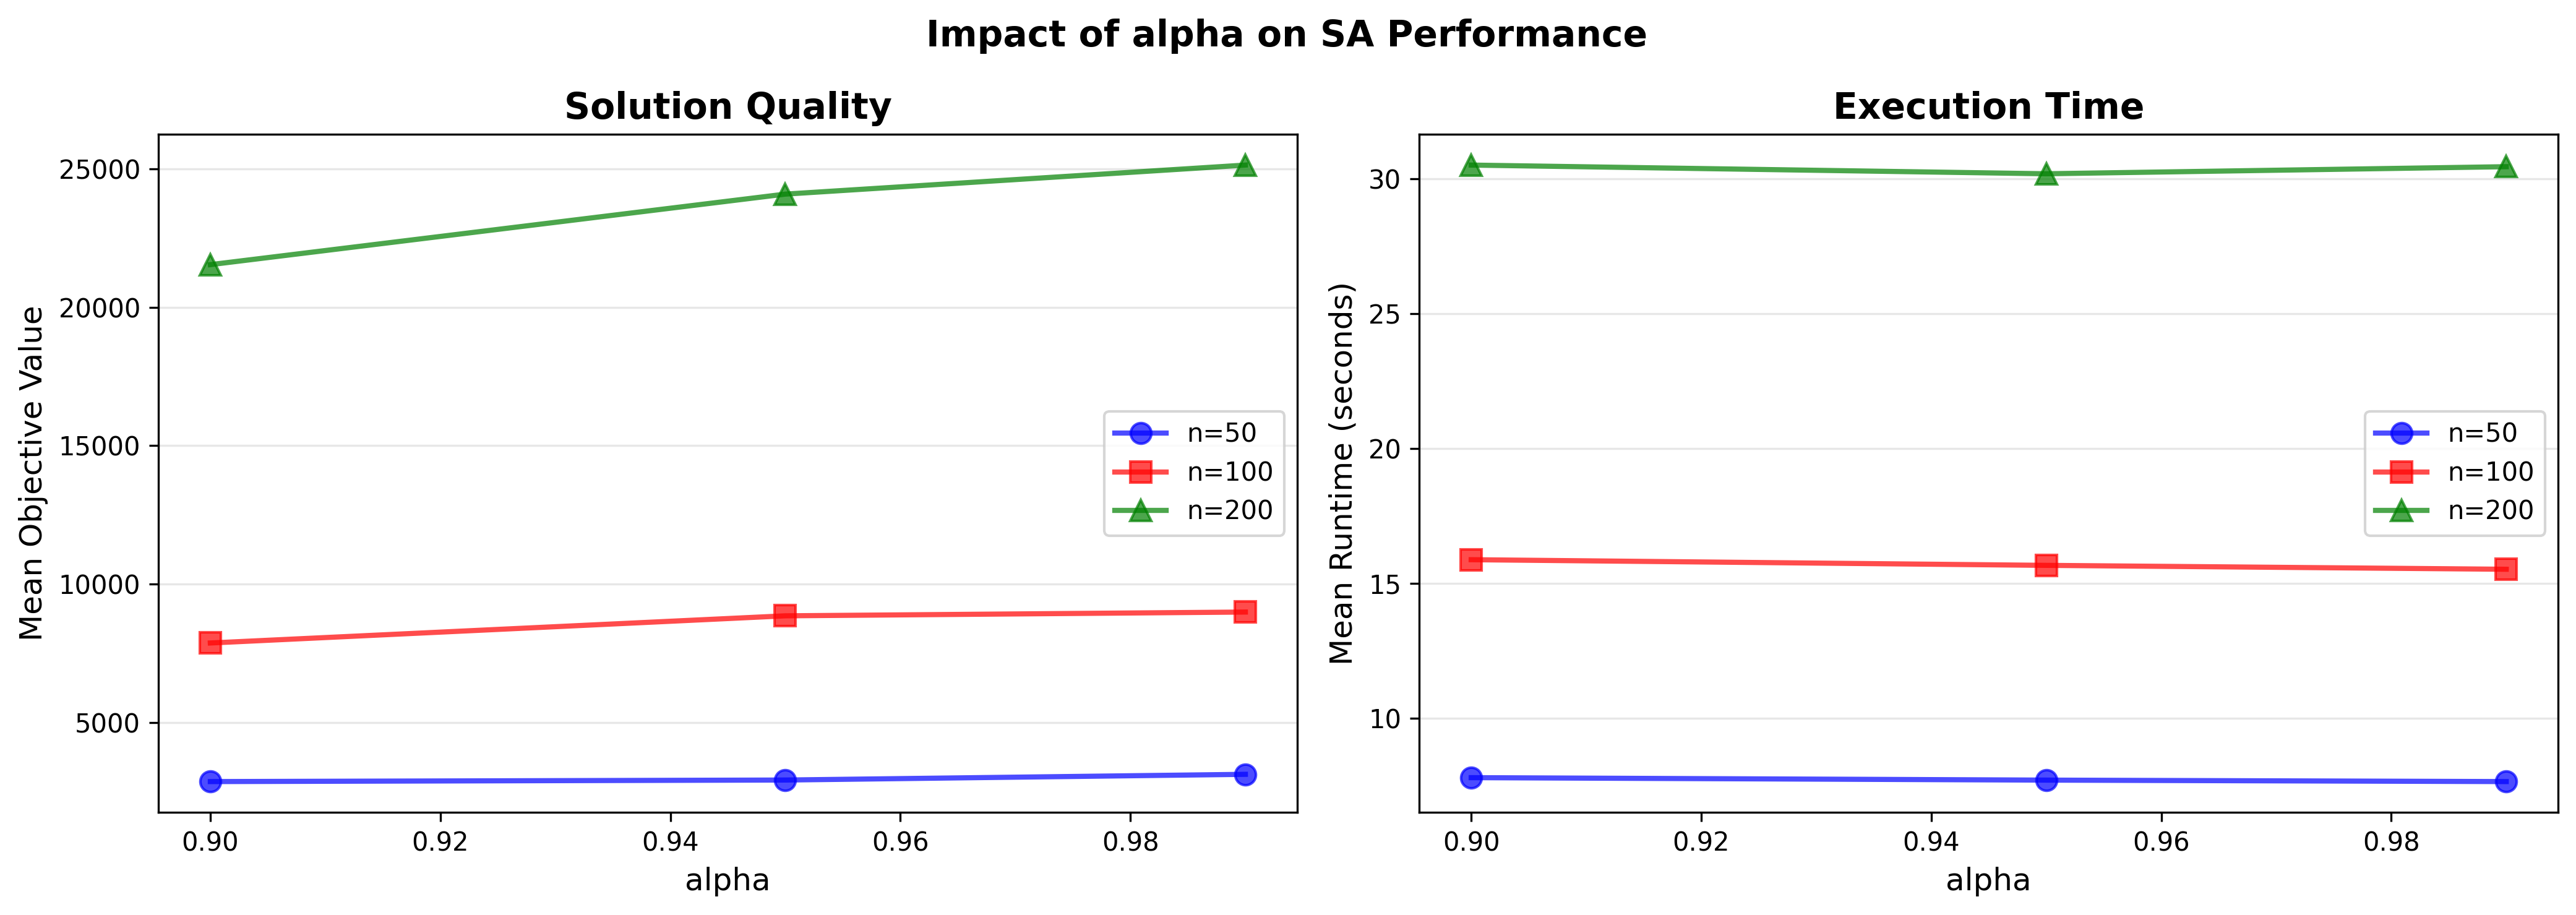
\includegraphics[width=1\linewidth]{impact_of_alpha_on_sa_performance_results_20251130_162817.png}
    \caption{SA Alpha Fine-Tuning}
    \label{fig:sa_alpha}
\end{figure}

\begin{figure}
    \centering
    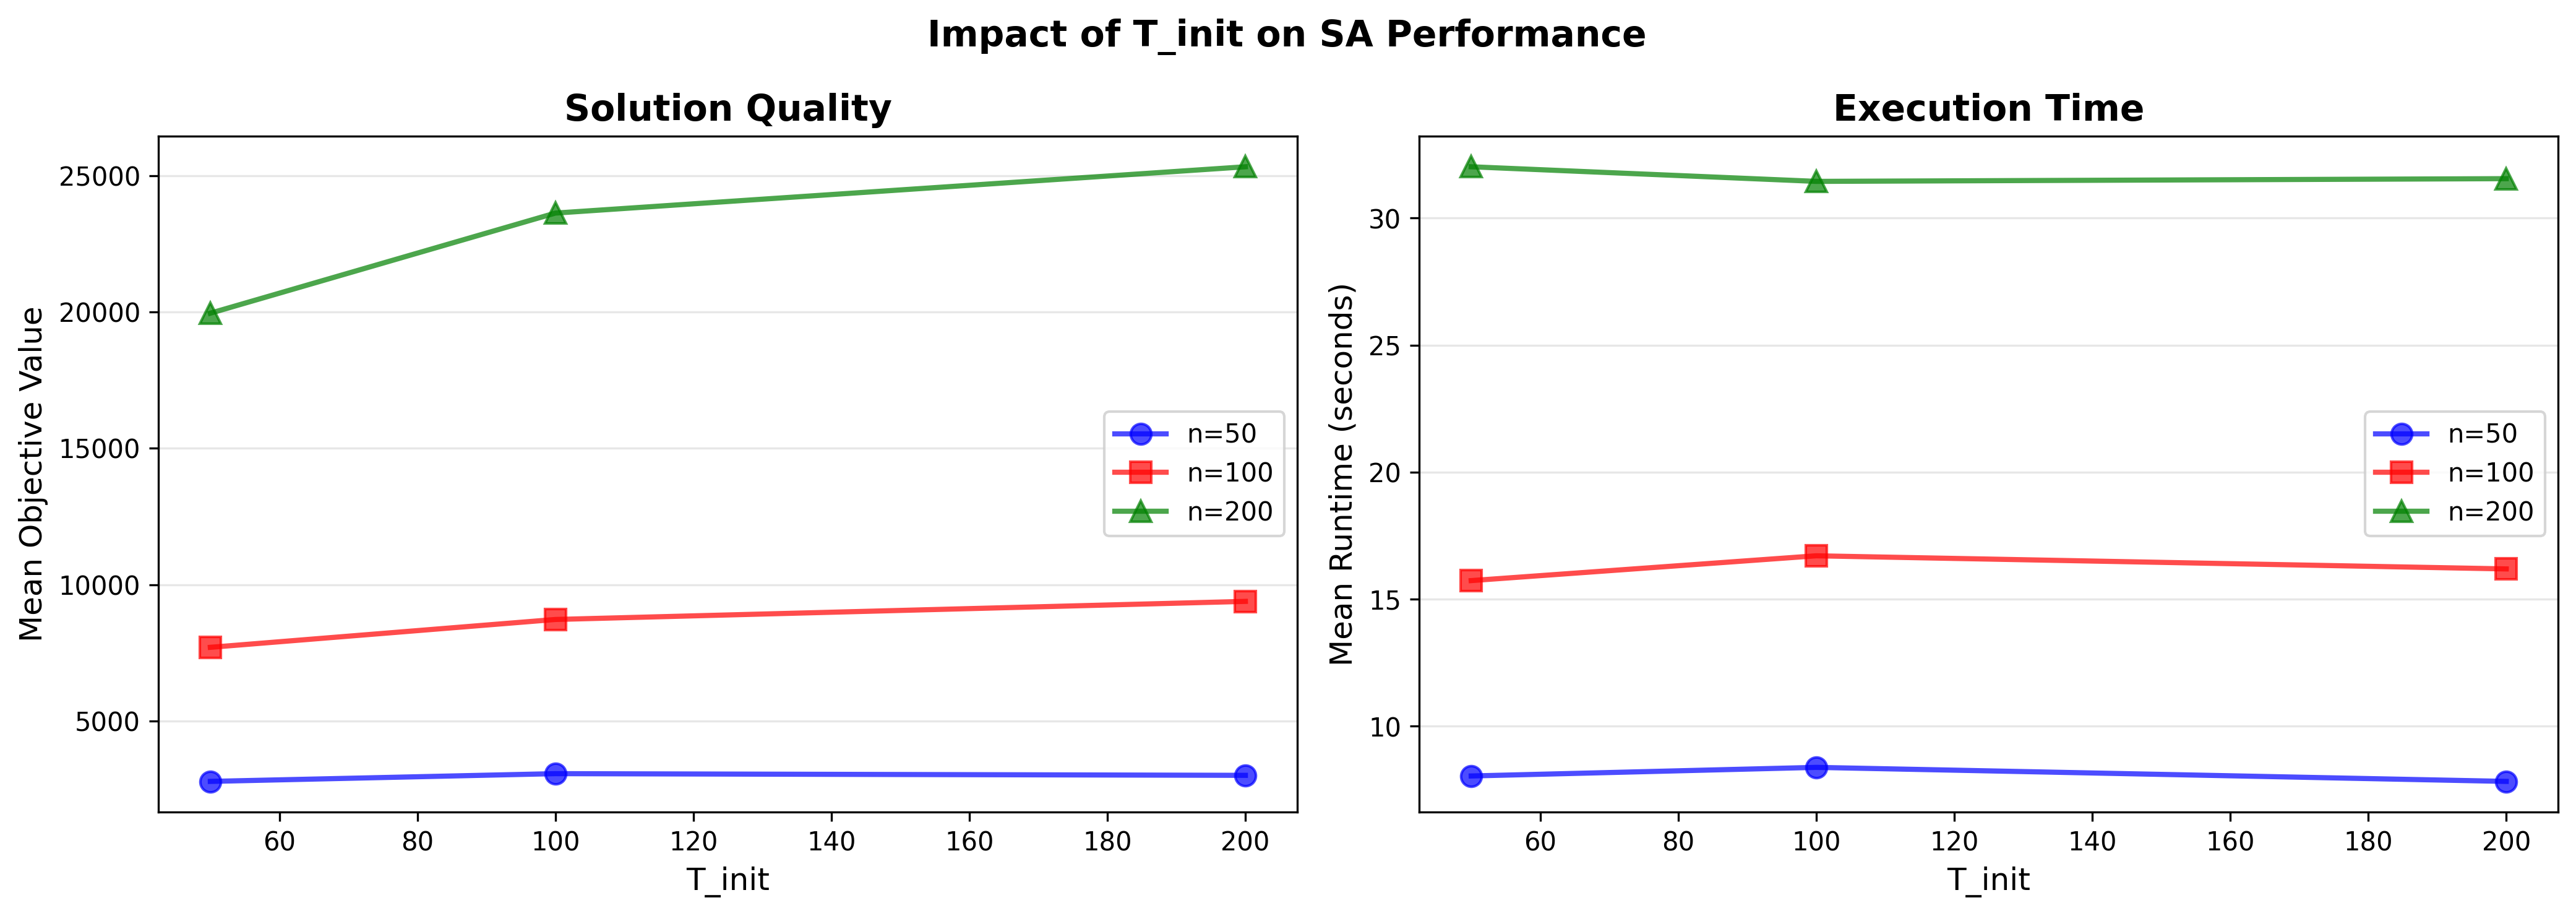
\includegraphics[width=1\linewidth]{impact_of_t_init_on_sa_performance_results_20251130_163641.png}
    \caption{SA Initial Temperature Fine-Tuning}
    \label{fig:sa_temperature}
\end{figure}

\begin{figure}
    \centering
    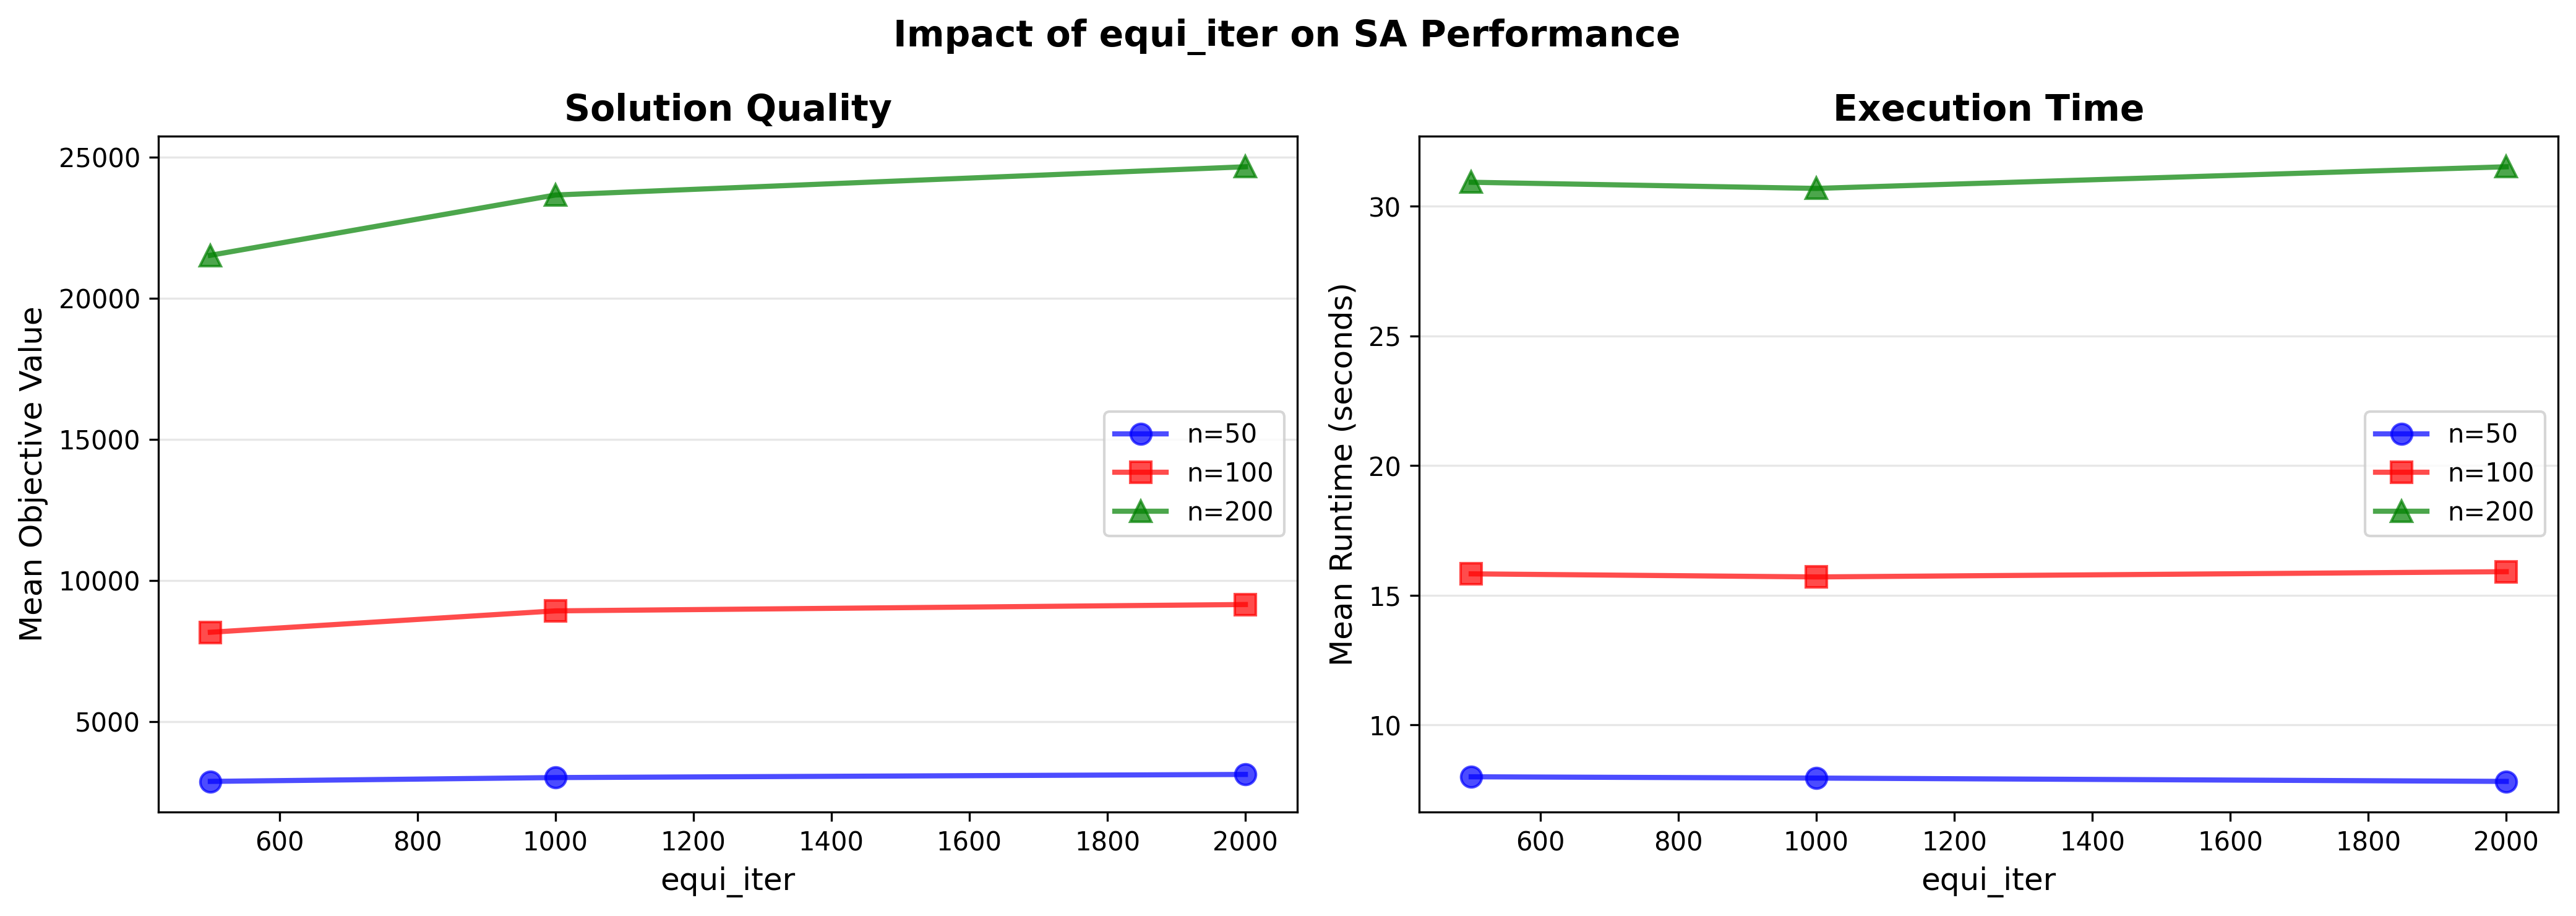
\includegraphics[width=1\linewidth]{impact_of_equi_iter_on_sa_performance_results_20251130_164455.png}
    \caption{SA Equilibrium Condition Fine-Tuning}
    \label{fig:sa_equi_iter}
\end{figure}

\subsection{Comparison of SA with Beam Search}
After experimenting with SA parameters the results felt off so we decided to compare this algorithm with another relatively strong algorithm to make sure it works correctly and it was clearly proved (especially on larger instances) as can be seen in Fig.~\ref{fig:sa_vs_beam}. SA outperformed Beam Search on every instance of size 100 and more with significant improvement in average objective value up to 35\% for instances of size 500.

\begin{figure}
    \centering
    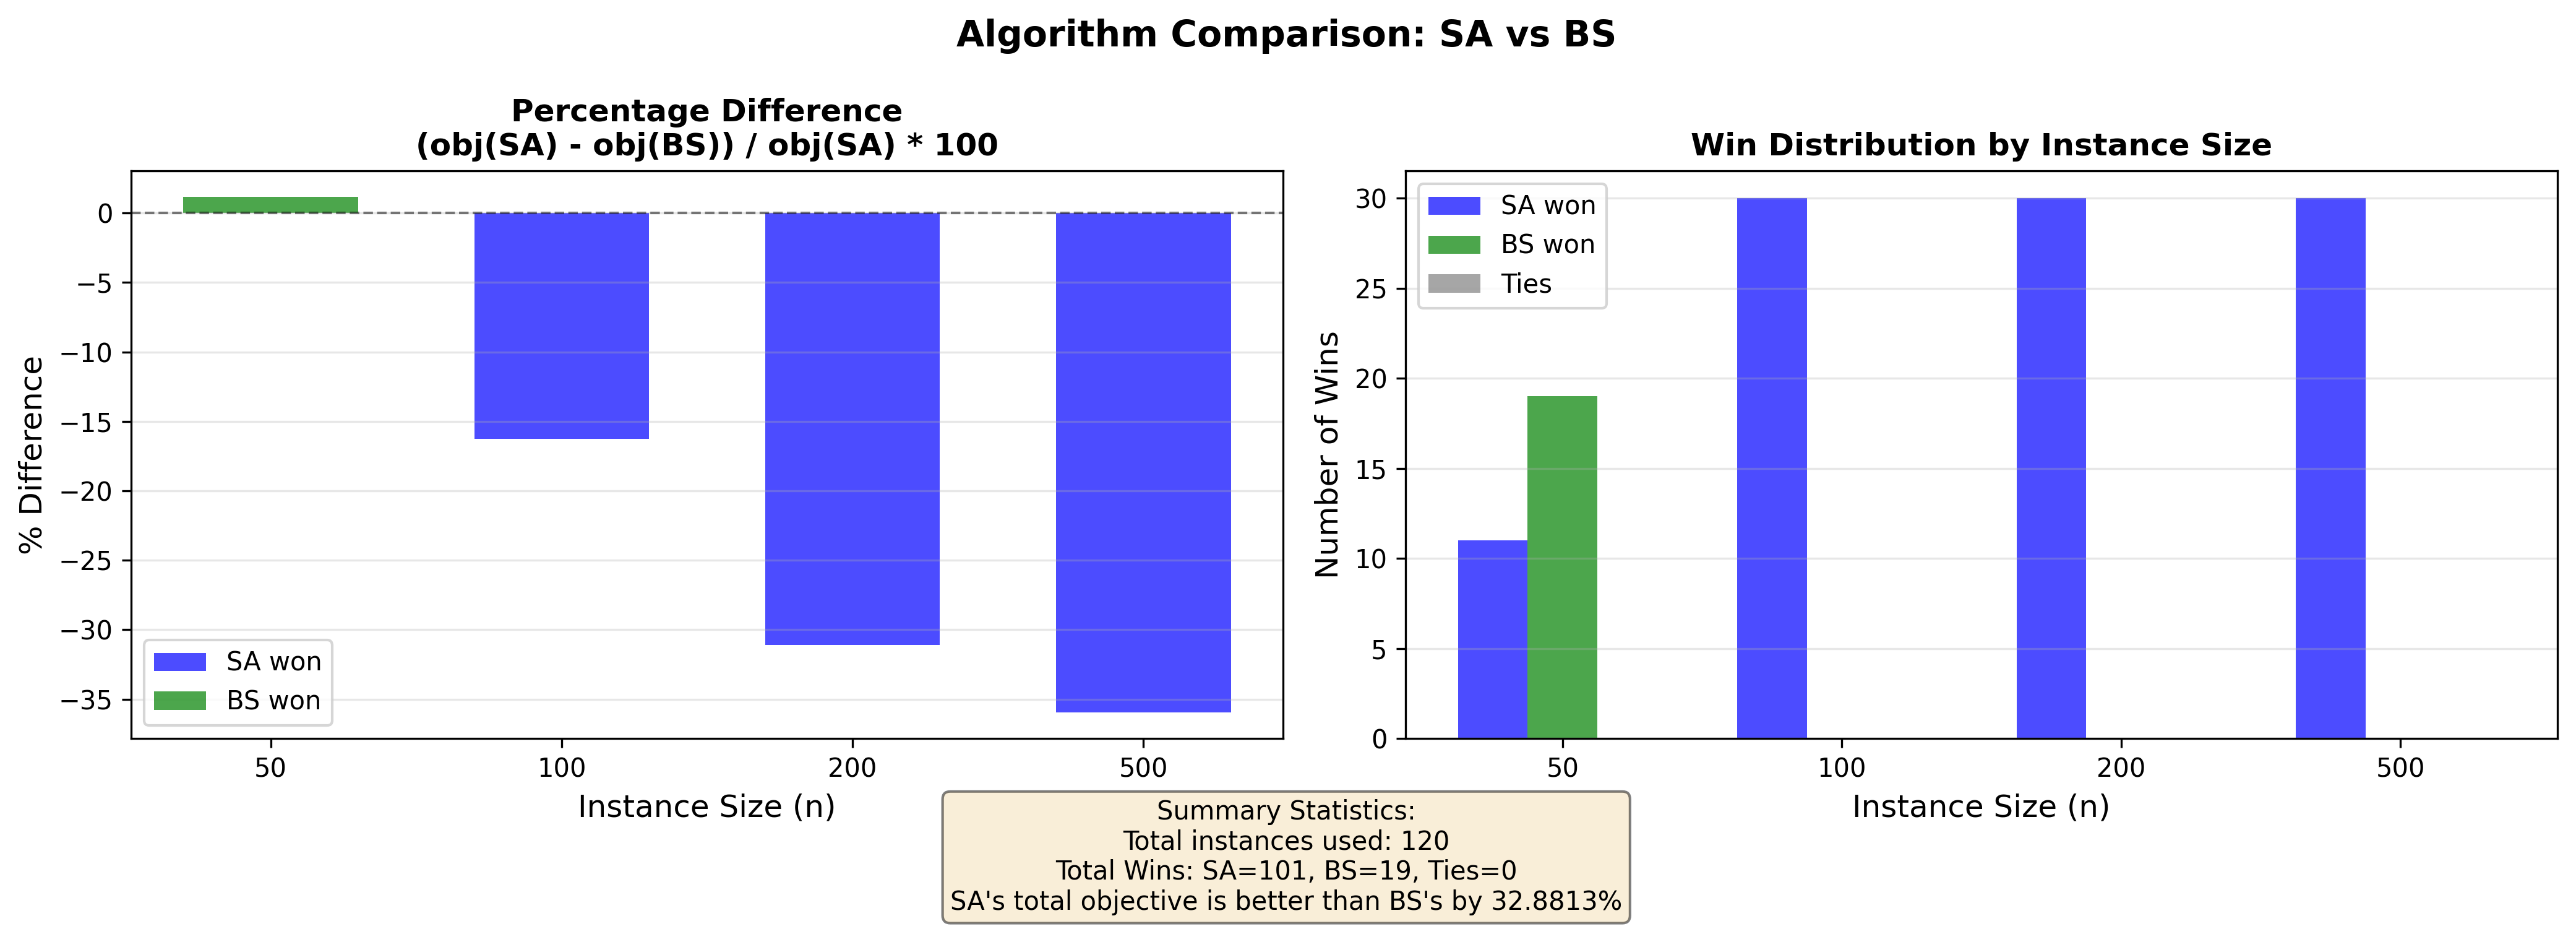
\includegraphics[width=1\linewidth]{SA_vs_BS_50-100-200-500_20251130_171513.png}
    \caption{Simulated Annealing vs Beam Search}
    \label{fig:sa_vs_beam}
\end{figure}



% ============================================================
% 10. Delta Evaluation
% ============================================================
\section{Delta Evaluation}

\subsection{Idea}
Delta evaluation is implemented in the \texttt{SCFPDPSolution} class to avoid redundant objective function computations during local search. The implementation maintains two cached values: total distance ($\sum d(R_k)$) and sum of squared distances ($\sum d(R_k)^2$), which are incrementally updated whenever a route is modified. The responsibilities distribution between \texttt{Route} and \texttt{SCFPDPSolution} classes is leveraged to simplify the flow of delta evaluation - \texttt{Route} is responsible for incrementally tracking distance of the route (similarly to TSP) while \texttt{SCFPDPSolution} only tracks total sum of distances and sum of squares for calculating the final objective value in $O(1)$. 

The delta evaluation mechanism uses a callback-based architecture. Each \texttt{Route} object holds a reference to the solution's \texttt{delta\_evaluation} callback method, which is invoked in \texttt{recompute\_route\_distance} whenever a route's changed. The callback receives both the new and old distance values, allowing incremental updates:

\begin{itemize}
\item cached\_total\_distance $\leftarrow$ cached\_total\_distance + ($new\_distance - old\_distance$)
\item cached\_sum\_of\_squares $\leftarrow$ cached\_sum\_of\_squares + ($new\_distance ^ 2 - old\_distance^2$)
\end{itemize}

Delta evaluation is employed by the method \texttt{recompute\_route\_distance} of the \texttt{Route} class whenever a change on the route is performed. This allows transparent continuous delta evaluation without the need to track the validity of the current objective value and related variables.

\subsection{Performance Analysis}

The objective function evaluation without delta evaluation requires iterating over all $K$ vehicles to compute the objective value and for each vehicle all locations of the route are calculated extensively. Even though the distance matrix is pre-calculated, the repetitive access to that matrix might be expensive, especially for larger instances where the matrix won't be able to get cached properly.

\begin{itemize}
  \item \textbf{Without delta evaluation:} $O(K)$ per objective computation (iterate over all routes to sum distances and squares)
  \item \textbf{With delta evaluation:} $O(1)$ per objective computation (direct access to cached values)
\end{itemize}

The performance improvement is most significant in local search contexts where objective evaluation dominates runtime:
\begin{itemize}
  \item Neighborhood size for swap/relocate operations: $O(n^2)$ where $n$ is the number of requests
  \item \texttt{BestImprovement} evaluates \emph{all} neighbors: $O(n^2)$ objective calls per iteration
  \item \textbf{Total complexity per local search iteration:}
  \begin{itemize}
      \item Without delta: $O(n^2 \cdot K)$
      \item With delta: $O(n^2)$
      \item \textbf{Speedup factor:} $K$ (number of vehicles)
  \end{itemize}
\end{itemize}

\subsection{Preprocessing}
The implementation leverages preprocessing through the precomputed distance matrix stored in the \\ \texttt{SCFPDPInstance} class. All pairwise Euclidean distances $\displaystyle d_{ij} = \lceil \sqrt{(x_i - x_j)^2 + (y_i - y_j)^2} \rceil$ are computed once during instance initialization and stored in $O(n^2)$ space. This preprocessing eliminates repeated square root, rounding operations and matrix access during route distance calculations, reducing the cost of \texttt{recompute\_route\_distance}.

\subsection{Experiments}
For assessing the impact of the delta evaluation on runtime, we have chosen beam search algorithm with branching factor of $5$ and $\beta = 3$ to have the algorithm explore $5$ different variations at every iteration. With this setup we have achieved a good balance between number of recalculations triggered during the solution construction and overall runtime of the experiment. The Fig.~\ref{fig:beam_delta_evaluation} displays the relative speedup of the delta evaluation for normalized visualization of the results per instance size over $3$ randomly sampled training instances of each size. On the left subplot we have measured the impact of branching factor on runtime with and without delta evaluation as branching factor is the main parameter in beam search that affects how many candidates are generated at each step and therefore how many times reevaluation is triggered. Both branching factor and instance size show the effect that delta evaluation has on the runtime as the instance grows. The speedup factor would be even higher if we used an algorithm that employs higher number of neighborhood moves and resulting objective recalculation. Another optimization that can be introduced to our solution - is lazy objective evaluation as it is designed in the \texttt{pymhlib}. For simplicity reasons we decided to implement eager recalculation at every route change assuming that the objective value is looked up after every step. 

\begin{figure}
    \centering
    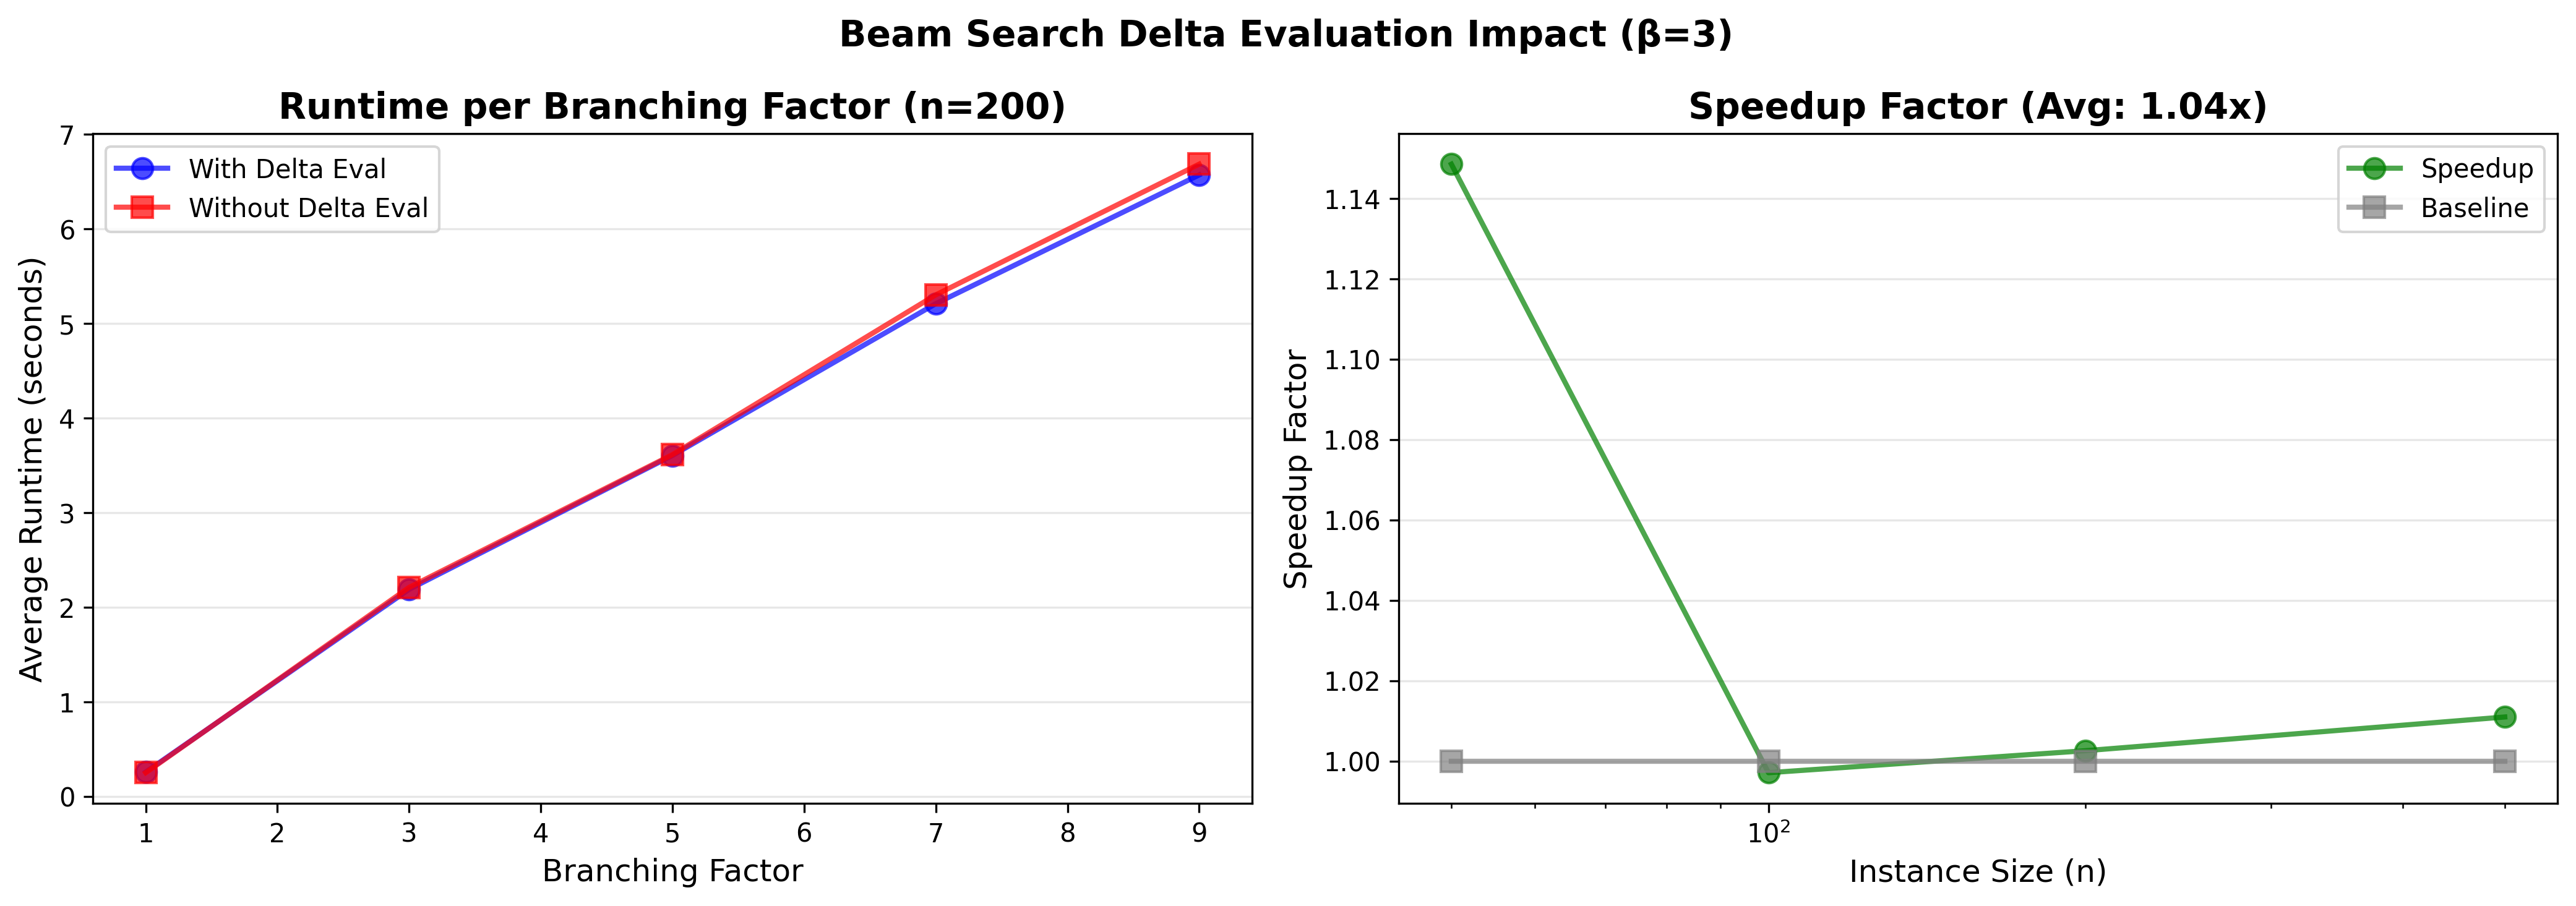
\includegraphics[width=1\linewidth]{beam_search_delta_evaluation_impact_(β=3)_results_20251130_143158.png}
    \caption{Delta Evaluation with Beam Search}
    \label{fig:beam_delta_evaluation}
\end{figure}

% ============================================================
% 11. Parameter Tuning}
% ============================================================
% \section{Parameter Tuning}
% \subsection{Neighborhood sizes}

% Include: small table of settings you tried.

% ============================================================
% 12. Results
% ============================================================
% \section{Results and Analysis}
% \subsection{Construction vs Randomized vs GRASP}
% \subsection{Local Search (6 variants)}
% \subsection{VND}
% \subsection{Plots}
% \begin{itemize}
%     \item Quality over time
%     \item Fairness trajectory
%     \item Travel duration trajectory
%     \item Boxplots over runs
% \end{itemize}


% ============================================================
% 13. Conclusions
% ============================================================
% \section{Conclusion}


% ============================================================
% Appendices
% ============================================================
% \appendix
% \section{Code Snippets}

% \begin{minted}{python}
% def vnd(v):
%     return v+1
% \end{minted}

% \section{Additional Plots}
% \section{Parameter Tables}

% --------------------
% \bibliographystyle{plain}

% \begin{thebibliography}{9}
% \bibitem{}
% \textit{},
% \url{}
% \end{thebibliography}

\end{document}